%# -*- coding: utf-8-unix -*-
%%==================================================
%% thesis.tex
%%==================================================

% 双面打印
\documentclass[bachelor, openright, twoside, english]{sjtuthesis}
% \documentclass[bachelor, openany, oneside, submit]{sjtuthesis}
% \documentclass[master, review]{sjtuthesis}
% \documentclass[%
%   bachelor|master|doctor|coursepaper, % 必选项,分别是学士,硕士,博士学位论文以及课程论文
%   fontset=fandol|windows|mac|ubuntu|adobe|founder, % 字体选项
%   oneside|twoside,        % 单面打印,双面打印(奇偶页交换页边距,默认)
%   openany|openright,      % 可以在奇数或者偶数页开新章|只在奇数页开新章(默认)
   % english,                % 启用英文模版
%   review,     % 盲审论文,隐去作者姓名、学号、导师姓名、致谢、发表论文和参与的项目
%   submit      % 定稿提交的论文,插入签名扫描版的原创性声明、授权声明
% ]

% 逐个导入参考文献数据库

% \usepackage[
%   separate-uncertainty = true,
%   multi-part-units = repeat
% ]{siunitx} 

\usepackage{hyperref}



\usepackage{url}  %Required
\usepackage{graphicx}  %Required
\usepackage{booktabs}
\usepackage{xspace}
\usepackage{color}
% \usepackage{subfig}
\usepackage{multirow}% http://ctan.org/pkg/multirow
\usepackage{hhline}% http://ctan.org/pkg/hhline
\usepackage[colorinlistoftodos]{todonotes}
\usepackage{siunitx}
\usepackage{amsfonts,amsthm,amsmath}
\usepackage{enumitem}
% \usepackage[belowskip=-15pt,aboveskip=0pt]{caption}
\usepackage[skip=2pt]{caption} % example skip set to 2pt
%\usepackage[belowskip=0pt,aboveskip=0pt]{caption}

% \setlength{\intextsep}{10pt plus 2pt minus 2pt}
\theoremstyle{definition}

\newtheorem{problem}{Problem}

\newcommand{\nop}[1]{}
\newcommand{\Todo}{{\textbf{\color{red}{todo-}}}}

% general terms for methods
\newcommand{\deepQLearning}{Deep Q-Learning\xspace}
\newcommand{\deepQNetwork}{Deep Q-Network\xspace}
\newcommand{\dqn}{DQN\xspace}

%notations
\newcommand{\notationFont}{\mathit}
\newcommand{\notationVec}{\mathbf}

\newcommand{\agent}{\notationFont{G}}
\newcommand{\agentVec}{\pmb{G}}
% \newcommand{\environment}{\notationFont{E}}
\newcommand{\environmentVec}{\notationVec{E}}
\newcommand{\user}{\notationFont{u}}
\newcommand{\action}{\notationFont{a}}
\newcommand{\actionVec}{\notationVec{a}}
\newcommand{\staterep}{\notationFont{s}}
\newcommand{\staterepVec}{\notationVec{S}}
\newcommand{\obervationrepVec}{\notationVec{O}}
\newcommand{\reward}{\notationFont{r}}
\newcommand{\rewardTotal}{\notationFont{R}}
\newcommand{\queueLength}{\notationFont{L}}
\newcommand{\numOfVehicles}{\notationFont{N}}
\newcommand{\distriOfVehicles}{\notationFont{D}}
\newcommand{\averageWaitingTime}{\notationFont{W}}
\newcommand{\image}{\notationFont{M}}
\newcommand{\phase}{\notationFont{p}}
\newcommand{\pressure}{\notationFont{P}}
\newcommand{\delay}{\notationFont{V}}
\newcommand{\switch}{\notationFont{C}}
\newcommand{\emergencyStop}{\notationFont{O}}
\newcommand{\numleft}{\notationFont{F}}
\newcommand{\durationleft}{\notationFont{D^F}}
\newcommand{\setOfVehicle}{\notationFont{J}}
\newcommand{\setOfLane}{\notationFont{I}}
\newcommand{\laneIndex}{\notationFont{i}}
\newcommand{\vehicleIndex}{\notationFont{j}}

\newcommand{\qnetwork}{\notationFont{Q}}
\newcommand{\expNotation}{\textsl}
\newcommand{\WE}{\expNotation{WE}\xspace}
\newcommand{\EW}{\expNotation{EW}\xspace}
\newcommand{\NS}{\expNotation{NS}\xspace}
\newcommand{\SN}{\expNotation{SN}\xspace}


\newcommand{\WEs}{\expNotation{WE-Straight}\xspace}
\newcommand{\WEl}{\expNotation{WE-Left}\xspace}
\newcommand{\SNs}{\expNotation{SN-Straight}\xspace}
\newcommand{\SNl}{\expNotation{SN-Left}\xspace}


\newcommand{\baselineNotation}{\textsf}
\newcommand{\FT}{\baselineNotation{FixedTime}\xspace}
\newcommand{\SOTL}{\baselineNotation{SOTL}\xspace}
\newcommand{\Greenwave}{\baselineNotation{GreenWave}\xspace}
\newcommand{\Maxpressure}{\baselineNotation{MaxPressure}\xspace}
\newcommand{\GWRL}{\baselineNotation{GWRL}\xspace}
\newcommand{\NIPS}{\baselineNotation{GRL}\xspace}
\newcommand{\Deeplight}{\baselineNotation{IntelliLight}\xspace}
% \newcommand{\PressLight}{\expNotation{PressLight-s}\xspace}
\newcommand{\base}{\baselineNotation{base}\xspace}
\newcommand{\SDeeplight}{\baselineNotation{base+seg}\xspace}
\newcommand{\NDeeplight}{\baselineNotation{base+neigh}\xspace}
\newcommand{\SNDeeplight}{\baselineNotation{base+neigh+seg}\xspace}
\newcommand{\PressLight}{\baselineNotation{PressLight}\xspace}
% \newcommand{\PressLight}{\expNotation{CTRL}\xspace}

\newcommand{\HeavyFlat}{{HeavyFlat}}
\newcommand{\HeavyPeak}{{HeavyPeak}}
\newcommand{\LightFlat}{{LightFlat}}
\newcommand{\LightPeak}{{LightPeak}}

\addbibresource{bib/thesis.bib}
% \addbibresource{bib/chap2.bib}

%# -*- coding: utf-8-unix -*-
% !TEX program = xelatex
% !TEX root = ../thesis.tex
% !TEX encoding = UTF-8 Unicode
%TC:ignore
\title{面向多路口交通信号灯控制的深度强化学习算法}
\author{陈诧姹}
\advisor{张伟楠}
% \coadvisor{某某教授}
\defenddate{2019年6月10日}
\coursename{某某课程}
\school{上海交通大学}
\institute{电子信息与电气工程学院}
\studentnumber{515021910302}
\cnacademicdegree{工学学士}
\major{计算机科学与技术}
\keywords{上海交大, 饮水思源, 爱国荣校}

\englishtitle{Deep reinforcement learning for multi-intersection traffic signal control}
\englishauthor{\textsc{Chacha Chen}}
\englishadvisor{Prof. \textsc{Weinan Zhang}}
% \englishcoadvisor{Prof. \textsc{Uom Uom}}
\englishschool{Shanghai Jiao Tong University}
\englishinstitute{\textsc{Depart of Computer Sience and Engineering, School of Electronic Information and Electrical Engineering} \\
  \textsc{Shanghai Jiao Tong University} \\
  \textsc{Shanghai, P.R.China}}
\englishinstitutemaster{Depart of Computer Sience and Engineering, \\ School of Electronic Information and Electrical Engineering}
\englishmajor{A Very Important Major}
\englishdate{Dec. 17th, 2014}
\enacademicdegree{Bachelor of Engineering}
\englishstudentid{515021910302}
\englishkeywords{SJTU, bachelor thesis, XeTeX/LaTeX template}
%TC:endignore
  % NOTE: the enclosed commands must be executed in preamble

\begin{document}

% 无编号内容:中英文论文封面、授权页
\maketitle
\makeatletter

\ifsjtu@coursepaper
% 摘要 部分课程论文需要,可以自行选择添加或者去除
% %# -*- coding: utf-8-unix -*-
% !TEX program = xelatex
% !TEX root = ../thesis.tex
% !TEX encoding = UTF-8 Unicode
%%==================================================
%% abstract.tex for SJTU Master Thesis
%%==================================================

\begin{abstract}


\end{abstract}

\begin{englishabstract}


\end{englishabstract}



% 目录 部分课程论文需要,可以自行选择添加或者去除
% \tableofcontents

\else
  \ifsjtu@submit\relax
    \includepdf{pdf/original.pdf}
    \cleardoublepage
    \includepdf{pdf/authorization.pdf}
    \cleardoublepage
  \else
    \ifsjtu@review\relax
    % exclude the original claim and authorization
    \else
      \makeDeclareOriginal
      \makeDeclareAuthorization
    \fi
  \fi
  \frontmatter % 使用罗马数字对前言编号

  % 摘要
  %# -*- coding: utf-8-unix -*-
% !TEX program = xelatex
% !TEX root = ../thesis.tex
% !TEX encoding = UTF-8 Unicode
%%==================================================
%% abstract.tex for SJTU Master Thesis
%%==================================================

\begin{abstract}


\end{abstract}

\begin{englishabstract}


\end{englishabstract}



  % 目录、插图目录、表格目录
  \tableofcontents
  \listoffigures
  \addcontentsline{toc}{chapter}{\listfigurename}     % 将插图目录加入全文目录
  \listoftables
  \addcontentsline{toc}{chapter}{\listtablename}      % 将表格目录加入全文目录
  \listofalgorithms
  \addcontentsline{toc}{chapter}{\listalgorithmname}  % 将算法目录加入全文目录

  \include{tex/symbol} % 主要符号、缩略词对照表
\fi

\makeatother
\mainmatter % 使用阿拉伯数字对正文编号

% 正文内容
% introduction.tex

\section{Introduction}
\label{sec:introduction}
Traffic congestion is a growing problem that continues to plague urban areas with negative outcomes to both the traveling public and society as a whole. These negative outcomes will only grow over time as more people flock to urban areas. In 2014, traffic congestion costs Americans over \$160 billion in lost productivity and wasted over 3.1 billion gallons of fuel~\cite{Econ14}. Traffic congestion was also attributed to over 56 billion pounds of harmful CO2 emissions in 2011~\cite{schrank20152015}. 
In the European Union, the cost of traffic congestion was equivalent to 1\% of the entire GDP~\cite{schrank2012tti}.
Mitigating congestion would have significant economic, environmental and societal benefits.
Signalized intersections are one of the most prevalent bottleneck types in urban environments, and thus traffic signal control plays a vital role in urban traffic management.

\begin{figure}[t]
\centering
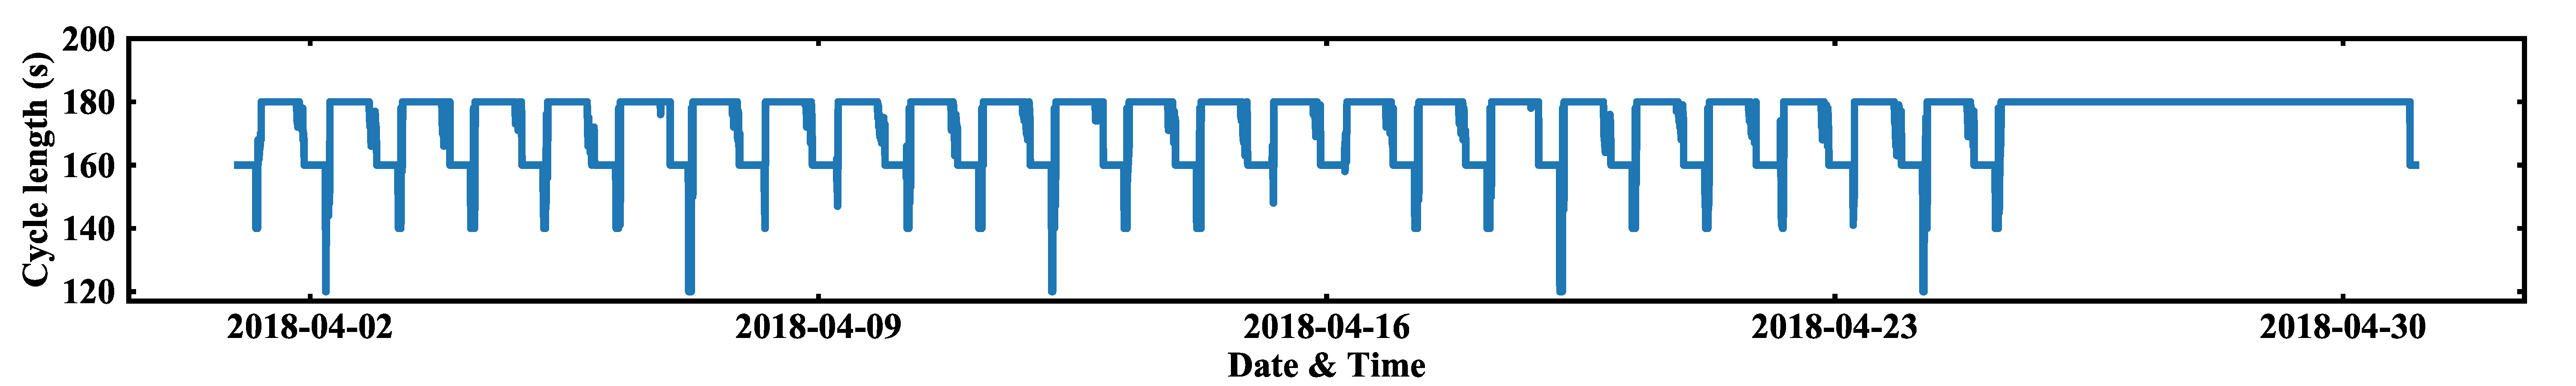
\includegraphics[width=0.99\textwidth]{figures/timing.pdf} 
\caption{Traffic signal timing in a city. The cycle length rarely changes.}
\label{fig:timing}
\end{figure}


\subsection{Current Situation}
In many modern cities today, the widely-used adaptive traffic signal control systems such as SCATS~\cite{SCATS} and SCOOT~\cite{hunt1981scoot,hunt1982scoot} heavily rely on manually designed traffic signal plans. Such manually set traffic signal plans are designed to be dynamically selected according to the traffic volume detected by loop sensors. However, many intersections do not have loop sensors installed or the loop sensors are poorly maintained. Moreover, the loop sensors are activated only when vehicles pass through them, thus they can only provide partial information about the vehicle through them. As a result, the signal cannot perceive and react to the real-time traffic patterns, and engineers need to manually change the traffic signal timings in the signal control system under certain traffic condition scenarios. Figure~\ref{fig:timing} shows the traffic signal timing at an intersection in a city of China and the traffic signal timing rarely changes regardless of the real traffic changes throughout the day.


\subsection{Opportunities}
\emph{First, today we have much richer information that can be collected from various sources.} Traditional traffic signal control relies on data from loop sensors, which can only sense the vehicle passing. However, new data sources are quickly becoming available that can serve as input for traffic signal control purposes. For instance, street-facing surveillance cameras used for security purposes can also provide a more detailed depiction of  the traffic situation on nearby roads -- specifically, how many cars are waiting in the lane, how many cars are taking turns, where they are located, and how fast they are traveling. In addition, large-scale trajectory data can be collected from various sources such as navigation applications (e.g., Google Maps),  ride-sharing platforms (e.g., Uber) and GPS-equipped vehicles that share information with the nearby infrastructure (e.g., connected vehicles). Such data provide us with more insight about how vehicles arrive to intersections. We have reached a stage of abundant mobility information that can describe the traffic dynamics in the city more clearly, which is an essential resource for us to improve the traffic control system.


 
\begin{figure}[htbp]
\centering
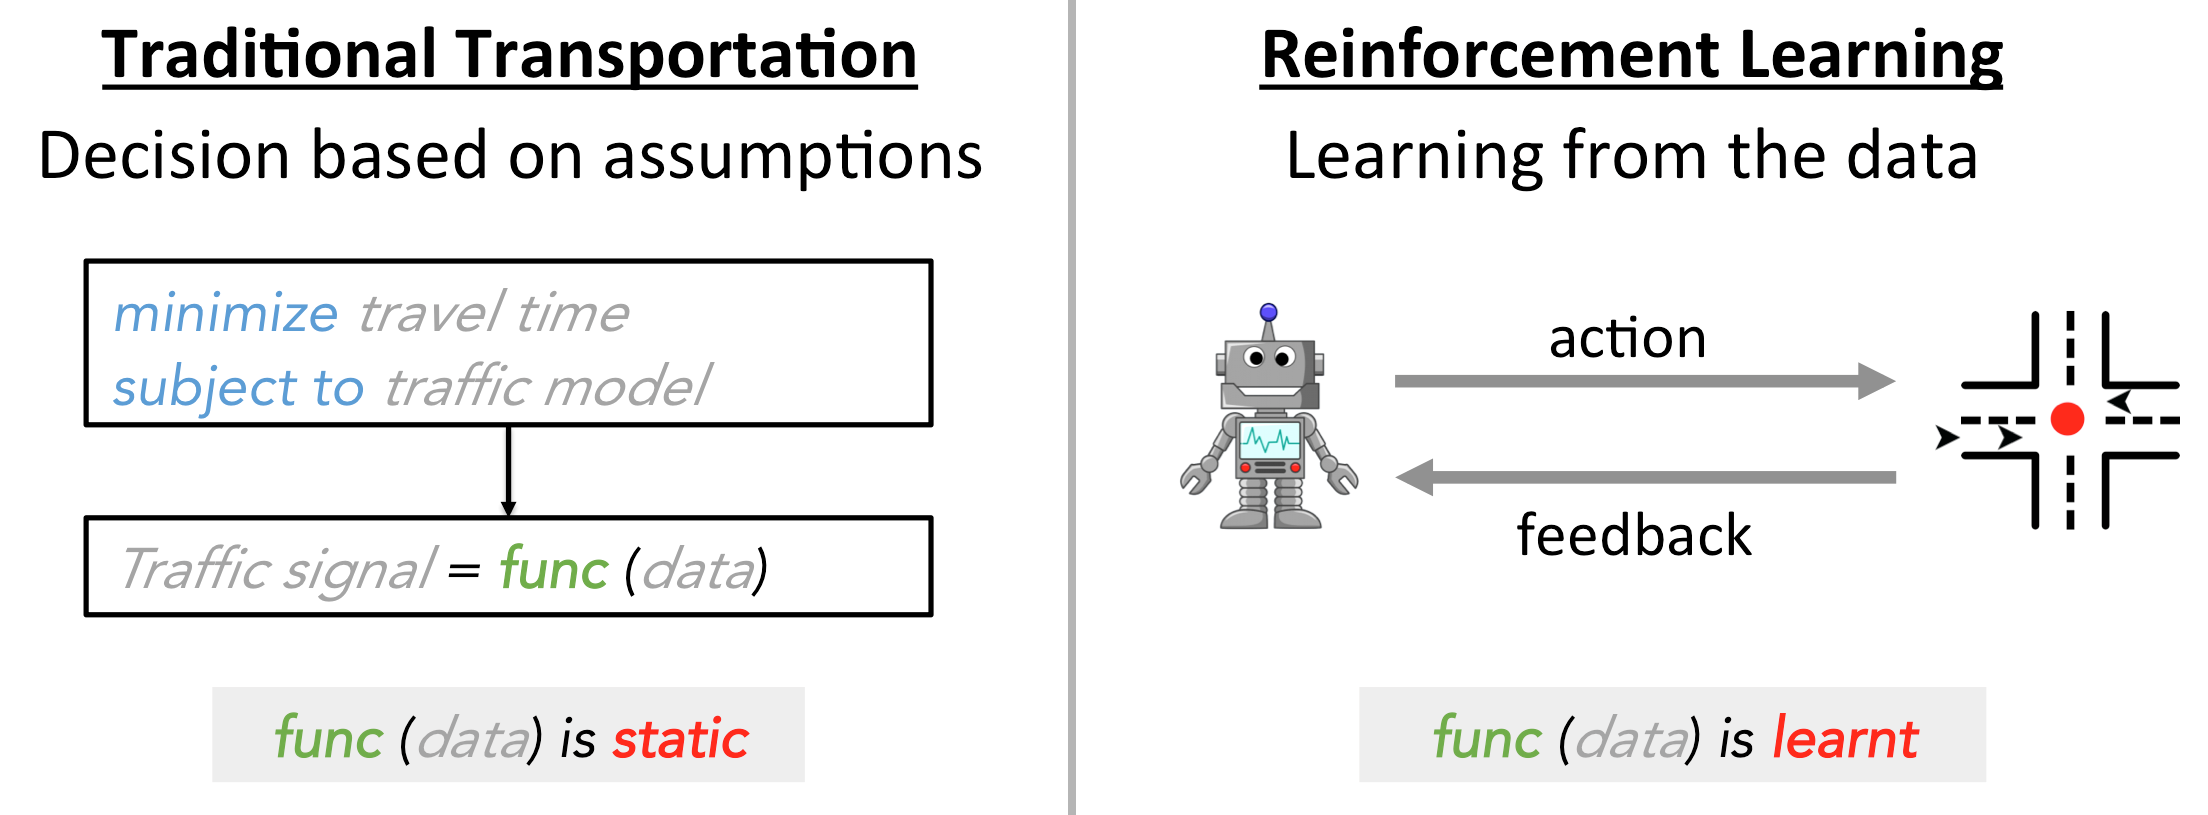
\includegraphics[width=0.7\columnwidth]{fig/optimizationvsRL.png}
\caption{Difference between traditional transportation approach and machine learning approach.}
\label{fig:optvsrl}
\end{figure}

\emph{Second, today we have much stronger computing power and advanced computational models.} The typical approach that transportation researchers take is to cast traffic signal control as an optimization problem under certain assumptions about the traffic model, e.g., vehicles come in a uniform and constant rate~\cite{RPM04}.  Various (and sometimes strong) assumptions have to be made in order to make the optimization problem tractable. The key issue here is that these assumptions deviate from the real world and often do so significantly. As we know, real-world traffic condition evolves in a complicated way, affected by many factors such as driver's preference, interactions with vulnerable road users (e.g. pedestrians, cyclists, etc.), weather and road conditions, just to name a few. These factors can hardly be fully described in a traffic model.


On the other hand, machine learning techniques can directly learn from the observed data without making unrealistic assumptions about the model. However, typical supervised learning does not apply here because existing traffic signal control systems follow pre-defined signal plans so we do not have enough training data to differentiate good and bad traffic signal plan strategies. Instead, we have to first take actions to change the signal plans and then learn from the outcomes. This trial-and-error approach is also the core idea of reinforcement learning (RL). In essence, an RL system generates and executes different strategies (e.g., for traffic signal control) based on the current environment. It will then learn and adjust the strategies based on the feedback from the environment. This reveals the biggest difference between transportation approaches and our RL approaches, which is illustrated in Figure~\ref{fig:optvsrl}: in traditional transportation research, the model $func(data)$ is static; in reinforcement learning, the model is dynamically learned through trial-and-error in the real environment.





% !TEX root = main.tex
% \chapter{Introduction}
% \label{chap:intro}

\chapter{Related Work}
\label{chap:related}
\textbf{Individual Traffic Signal Control.}
Individual traffic signal control has been investigated extensively in the field of transportation. These methods try to optimize the travel time or delay of vehicles~\cite{Gart83,Henr84,Boil06,SeHe97,Liang18}, building on the assumption that vehicles are arriving and moving in a specific pattern. Recently, reinforcement learning based methods attempt to address this problem by directly learning from the data~\cite{Wier00,MaDH16}. Earlier work using tabular Q-learning~\cite{APK03,ElAb10} can only deal with discrete state representations. Recent work using deep Q-learning~\cite{liLW16,VaOl16,wei2018intellilight} and policy gradient~\cite{MSCH17,Casa17PG} can cope with more complex continuous state representation, and hence have shown better performance.

\textbf{Conventional Multi-intersection Traffic Signal Control.}
Conventional multi-intersection control usually requires the intersections to have the same cycle length, coordination can be achieved by setting a fixed offset (i.e., the time interval between the beginnings of green lights) among all intersections~\cite{urbanik2015signal} in grid networks with homogeneous blocks. In fact, it is not an easy task to even provide coordination along an arterial, given traffic of opposite directions usually cannot be facilitated simultaneously. To solve this problem, some optimization-based methods~\cite{robertson1969transyt,little1981maxband} are developed to minimize vehicle travel time and/or the number of stops at multiple intersections. 
Systems like SCATS and SCOOT also have internal selection or optimization processes to modify cycle length, phase splits and offsets ~\cite{kergaye2010comparative}. Instead of optimizing offsets, max-pressure~\cite{MP13,MP13book} aims to maximize throughput of the network so as to minimizing the travel time. However, these approaches still rely on assumptions to simplify the traffic condition, and do not guarantee optimal results in the real world.

\textbf{RL-based Multi-intersection Traffic Signal Control.}
Since recent advances in RL improve the performance on isolated traffic signal control~\cite{VaOl16,wei2018intellilight}, efforts have been made to design strategies that control multiple intersections. \textit{One way} is to consider explicit coordination mechanisms between learning agents using coordination graphs\cite{KWBV08,VaOl16}, extending \cite{Wier00} using max-plus algorithm. Since all the above methods need to negotiate between the agents in the whole network, they are computationally expensive. \textit{Another way} is to use individual RL agents to control the traffic signals in the multi-intersection system~\cite{ElAA13,ALUK10,da2006adaptive}. These methods are more scalable, since each agent makes its own decision based on the information from itself and neighboring intersections without explicit coordination. Our proposed method also follows this direction. However, none of the existing studies draw a connection with traditional transportation methods. 

%they only focus on rewards and overlook the adaptability of the algorithms to the real traffic. Therefore, they cannot interpret why the learned light signal changes corresponding to the traffic. In this paper, we try to test the algorithms in different traffic setting, and add more interpretation other than just reward.

\nop{
Conventional control methods in isolated intersections use closed-form solutions given by optimization of operational parameters based on assumptions and constraints, while reinforcement learning methods have proven useful in this problem as they are able to learn from data collected from sensors in a more intelligent and adaptive way. \Todo-Guanjie, make it shorter


\begin{itemize}
\item Coordinated method
\item non-Coordinated method
\item centralized control(searching space)
\end{itemize}

Isolated traffic signal control has been investigated extensively in the field of transportation. These methods try to optimize the travel time or delay of vehicles~\cite{Gart83,Henr84,Boil06,SeHe97}, building on the assumption that vehicles are arriving and moving in a specific pattern. Recently, reinforcement learning based methods attempt to attack this problem by directly learning from the data~\cite{wiering2000multi,mannion2016experimental}. Earlier work using tabular Q-learning~\cite{APK03,ElAb10} can only deal with discrete state representations. Recent work using deep Q-learning~\cite{li2016traffic,van2016coordinated,wei2018intellilight} and policy gradient~\cite{mousavi_traffic_2017,mousavi_traffic_2017} can cope with more complex continuous state representation, and hence have shown better performance.

However, major challenges lie in the control of multi-intersection scenario, i.e., along an arterial and inside a network. Current methods generally have two categories, centralized methods, and decentralized methods~\cite{SQAS15}. 


Centralized methods are implemented either with pre-defined or with traffic-responsive methods, while both of them are not easy to scale.  Pre-defined centralized approaches usually use historical data to calculate splits and cycle times so as to maximize the flow in a specific direction. One of the widely-used pre-defined centralized coordinated methods in transportation engineering is through "Green Wave", i.e., vehicle will see a progressive cascade of green lights, to optimize the travel time of vehicles along an arterial. The problem with fixed coordination is that the solution is based on an aggregated average traffic pattern, and therefore does not necessarily address real-time situations satisfactorily. Traffic responsive centralized systems, on the other hand, use a centralized agent to control all intersections for the sake of coordination. Each intersection is typically controlled by traffic-responsive methods for changing signal phases. For systems like SCATS or SCOOT, the decisions are made after internal selection and optimization inside the control systems, which may not reflect real-world consequences. \todo{ZY will work on this part}Centralized methods work well only with well-defined traffic volume patterns. In cities where these patterns are not clearly separable (e.g., cities where business centers are no longer located exclusively downtown), coordination may not be effective. What's more, when adding new intersections into the system, centralized methods are not easy to scale, since it may require a large number of central updates of control strategies, or even learning from scratch. 

\nop{Isolated traffic responsive systems, on the other hand, use inductive loop sensors to determine if there is a long queue of stopped cars, but this decision is only locally optimal.
\todo{In both SCATS and SCOOT systems there are coordination between intersections. Maybe say "the decisions are made after internal selection and optimization inside the control systems, which may not reflect real-world consequences"}

In this sense, traffic responsive coordinated control may have a better performance. One type of solution is centralized methods which requires a centralized agent to control all intersections for the sake of coordination. Each intersection is typically controlled by fixed-time plans for changing signal phases, which is largely reply \todo{dependent?} on prior knowledge. For systems like SCATS or SCOOT, the baseline plans of signal settings are predetermined based on engineering experience. This approach works well only in traffic networks with well defined traffic volume patterns\todo{these adaptive methods  do address changes in traffic}. In cities where these patterns are not clearly separable (e.g., cities where business centers are no longer located exclusively downtown), coordination may not be effective. What's more, when adding new intersections into the system, centralized methods are not easy to scale, since it may require a large number of central updates of control strategies, or even learning from scratch. 
}

In this sense, decentralized methods may be more scalable and practicable. Decentralized methods make use of isolated traffic signal control methods, using the information from both target and surrounding intersections. They are computationally less demanding because they only need and maintain relevant information from surrounding intersections/controllers. By plugging new intersection controllers into the system, the decentralized systems are easy to scale. 

However, decentralized methods assume relatively static traffic environments, and are hence far from the real case. What's more, they only focus on rewards and overlook the adaptability of the algorithms
to the real traffic. Therefore, they cannot interpret why the learned light signal changes corresponding to the traffic. In this paper, we try to test the algorithms in different traffic settings and add more interpretations other than reward. As far as we know, it is the first time that the policy learned by the reinforcement learning control agents are interpreted using the traditional transportation coordination method on an arterial.

\nop{Multi-intersection traffic light control has attracted a lot of attention in recent years due to its essential role in adjusting traffic. Current methods generally have two categories, centralized methods, and de-centralized methods. 

Centralized methods use a centralized agent to control all intersections for the sake of cooperation. Each intersection is typically controlled by fixed-time plans for changing signal phases, which is largely reply on prior knowledge. For systems like SCATS or SCOOT, the cooperation rules are defined by human experts (based on ). These rules do not adapt to dynamically changing traffic in real time. 

In general, centralized methods and systems can not scale to large arterials. Traditional centralized systems are usually designed around the larger scale, therefore, adding some controllers requires a large number of central updates of computers and softwares. The operation is relatively complicated and the operator must adjust many parameters. The maintenance of highly skilled and trained operators is expensive.


Decentralized systems rely on the control strategies of individual signal. They are computationally less demanding because they only need and maintain relevant information from surrounding intersections/controllers.

By plugging new controllers into the system, distributed systems are scalable and easy to scale.

The establishment and operation of a decentralized system is often inexpensive because there is no need for a reliable and direct communication network between the central computer and the local controller in the field. As a result, inexpensive communication alternatives such as wireless communication networks have created viable options that significantly reduce system cost}
}

% \input{introduction}
% % !TEX root = main.tex
% \chapter{Introduction}
% \label{chap:intro}

\chapter{Related Work}
\label{chap:related}
\textbf{Individual Traffic Signal Control.}
Individual traffic signal control has been investigated extensively in the field of transportation. These methods try to optimize the travel time or delay of vehicles~\cite{Gart83,Henr84,Boil06,SeHe97,Liang18}, building on the assumption that vehicles are arriving and moving in a specific pattern. Recently, reinforcement learning based methods attempt to address this problem by directly learning from the data~\cite{Wier00,MaDH16}. Earlier work using tabular Q-learning~\cite{APK03,ElAb10} can only deal with discrete state representations. Recent work using deep Q-learning~\cite{liLW16,VaOl16,wei2018intellilight} and policy gradient~\cite{MSCH17,Casa17PG} can cope with more complex continuous state representation, and hence have shown better performance.

\textbf{Conventional Multi-intersection Traffic Signal Control.}
Conventional multi-intersection control usually requires the intersections to have the same cycle length, coordination can be achieved by setting a fixed offset (i.e., the time interval between the beginnings of green lights) among all intersections~\cite{urbanik2015signal} in grid networks with homogeneous blocks. In fact, it is not an easy task to even provide coordination along an arterial, given traffic of opposite directions usually cannot be facilitated simultaneously. To solve this problem, some optimization-based methods~\cite{robertson1969transyt,little1981maxband} are developed to minimize vehicle travel time and/or the number of stops at multiple intersections. 
Systems like SCATS and SCOOT also have internal selection or optimization processes to modify cycle length, phase splits and offsets ~\cite{kergaye2010comparative}. Instead of optimizing offsets, max-pressure~\cite{MP13,MP13book} aims to maximize throughput of the network so as to minimizing the travel time. However, these approaches still rely on assumptions to simplify the traffic condition, and do not guarantee optimal results in the real world.

\textbf{RL-based Multi-intersection Traffic Signal Control.}
Since recent advances in RL improve the performance on isolated traffic signal control~\cite{VaOl16,wei2018intellilight}, efforts have been made to design strategies that control multiple intersections. \textit{One way} is to consider explicit coordination mechanisms between learning agents using coordination graphs\cite{KWBV08,VaOl16}, extending \cite{Wier00} using max-plus algorithm. Since all the above methods need to negotiate between the agents in the whole network, they are computationally expensive. \textit{Another way} is to use individual RL agents to control the traffic signals in the multi-intersection system~\cite{ElAA13,ALUK10,da2006adaptive}. These methods are more scalable, since each agent makes its own decision based on the information from itself and neighboring intersections without explicit coordination. Our proposed method also follows this direction. However, none of the existing studies draw a connection with traditional transportation methods. 

%they only focus on rewards and overlook the adaptability of the algorithms to the real traffic. Therefore, they cannot interpret why the learned light signal changes corresponding to the traffic. In this paper, we try to test the algorithms in different traffic setting, and add more interpretation other than just reward.

\nop{
Conventional control methods in isolated intersections use closed-form solutions given by optimization of operational parameters based on assumptions and constraints, while reinforcement learning methods have proven useful in this problem as they are able to learn from data collected from sensors in a more intelligent and adaptive way. \Todo-Guanjie, make it shorter


\begin{itemize}
\item Coordinated method
\item non-Coordinated method
\item centralized control(searching space)
\end{itemize}

Isolated traffic signal control has been investigated extensively in the field of transportation. These methods try to optimize the travel time or delay of vehicles~\cite{Gart83,Henr84,Boil06,SeHe97}, building on the assumption that vehicles are arriving and moving in a specific pattern. Recently, reinforcement learning based methods attempt to attack this problem by directly learning from the data~\cite{wiering2000multi,mannion2016experimental}. Earlier work using tabular Q-learning~\cite{APK03,ElAb10} can only deal with discrete state representations. Recent work using deep Q-learning~\cite{li2016traffic,van2016coordinated,wei2018intellilight} and policy gradient~\cite{mousavi_traffic_2017,mousavi_traffic_2017} can cope with more complex continuous state representation, and hence have shown better performance.

However, major challenges lie in the control of multi-intersection scenario, i.e., along an arterial and inside a network. Current methods generally have two categories, centralized methods, and decentralized methods~\cite{SQAS15}. 


Centralized methods are implemented either with pre-defined or with traffic-responsive methods, while both of them are not easy to scale.  Pre-defined centralized approaches usually use historical data to calculate splits and cycle times so as to maximize the flow in a specific direction. One of the widely-used pre-defined centralized coordinated methods in transportation engineering is through "Green Wave", i.e., vehicle will see a progressive cascade of green lights, to optimize the travel time of vehicles along an arterial. The problem with fixed coordination is that the solution is based on an aggregated average traffic pattern, and therefore does not necessarily address real-time situations satisfactorily. Traffic responsive centralized systems, on the other hand, use a centralized agent to control all intersections for the sake of coordination. Each intersection is typically controlled by traffic-responsive methods for changing signal phases. For systems like SCATS or SCOOT, the decisions are made after internal selection and optimization inside the control systems, which may not reflect real-world consequences. \todo{ZY will work on this part}Centralized methods work well only with well-defined traffic volume patterns. In cities where these patterns are not clearly separable (e.g., cities where business centers are no longer located exclusively downtown), coordination may not be effective. What's more, when adding new intersections into the system, centralized methods are not easy to scale, since it may require a large number of central updates of control strategies, or even learning from scratch. 

\nop{Isolated traffic responsive systems, on the other hand, use inductive loop sensors to determine if there is a long queue of stopped cars, but this decision is only locally optimal.
\todo{In both SCATS and SCOOT systems there are coordination between intersections. Maybe say "the decisions are made after internal selection and optimization inside the control systems, which may not reflect real-world consequences"}

In this sense, traffic responsive coordinated control may have a better performance. One type of solution is centralized methods which requires a centralized agent to control all intersections for the sake of coordination. Each intersection is typically controlled by fixed-time plans for changing signal phases, which is largely reply \todo{dependent?} on prior knowledge. For systems like SCATS or SCOOT, the baseline plans of signal settings are predetermined based on engineering experience. This approach works well only in traffic networks with well defined traffic volume patterns\todo{these adaptive methods  do address changes in traffic}. In cities where these patterns are not clearly separable (e.g., cities where business centers are no longer located exclusively downtown), coordination may not be effective. What's more, when adding new intersections into the system, centralized methods are not easy to scale, since it may require a large number of central updates of control strategies, or even learning from scratch. 
}

In this sense, decentralized methods may be more scalable and practicable. Decentralized methods make use of isolated traffic signal control methods, using the information from both target and surrounding intersections. They are computationally less demanding because they only need and maintain relevant information from surrounding intersections/controllers. By plugging new intersection controllers into the system, the decentralized systems are easy to scale. 

However, decentralized methods assume relatively static traffic environments, and are hence far from the real case. What's more, they only focus on rewards and overlook the adaptability of the algorithms
to the real traffic. Therefore, they cannot interpret why the learned light signal changes corresponding to the traffic. In this paper, we try to test the algorithms in different traffic settings and add more interpretations other than reward. As far as we know, it is the first time that the policy learned by the reinforcement learning control agents are interpreted using the traditional transportation coordination method on an arterial.

\nop{Multi-intersection traffic light control has attracted a lot of attention in recent years due to its essential role in adjusting traffic. Current methods generally have two categories, centralized methods, and de-centralized methods. 

Centralized methods use a centralized agent to control all intersections for the sake of cooperation. Each intersection is typically controlled by fixed-time plans for changing signal phases, which is largely reply on prior knowledge. For systems like SCATS or SCOOT, the cooperation rules are defined by human experts (based on ). These rules do not adapt to dynamically changing traffic in real time. 

In general, centralized methods and systems can not scale to large arterials. Traditional centralized systems are usually designed around the larger scale, therefore, adding some controllers requires a large number of central updates of computers and softwares. The operation is relatively complicated and the operator must adjust many parameters. The maintenance of highly skilled and trained operators is expensive.


Decentralized systems rely on the control strategies of individual signal. They are computationally less demanding because they only need and maintain relevant information from surrounding intersections/controllers.

By plugging new controllers into the system, distributed systems are scalable and easy to scale.

The establishment and operation of a decentralized system is often inexpensive because there is no need for a reliable and direct communication network between the central computer and the local controller in the field. As a result, inexpensive communication alternatives such as wireless communication networks have created viable options that significantly reduce system cost}
}

\chapter{PressLight: Learning Max Pressure Control for Signalized Intersections in Arterial Network}
\label{chap:presslight}
\section{Overview}
\label{sec:intro}


Traffic signals coordinate the traffic movements at the intersection and a smart traffic signal control algorithm is the key to transportation efficiency. Traffic signal control remains an active research topic because of the high complexity of the problem. The traffic situations are highly dynamic, thus require traffic signal plans to be able to adjust to different situations.

Recently, people start to investigate reinforcement learning (RL) techniques for traffic signal control. Several studies have shown the superior performance of RL techniques over traditional transportation approaches~\cite{Wier00,AbPK03,ALUK10,AbMB13,VaOl16,wei2018intellilight}. The biggest advantage of RL is that it directly learns how to take the next actions by observing the feedback from the environment after previous actions. 

\begin{figure}[]
\centering
\begin{tabular}{ccc}
   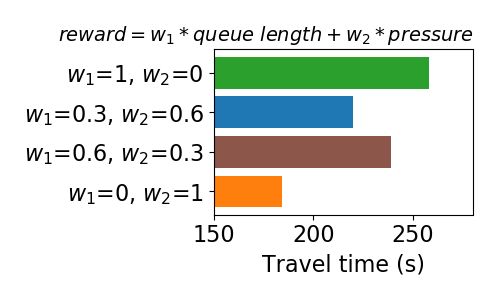
\includegraphics[width=0.45\textwidth]{figures/intro_1.png}&
   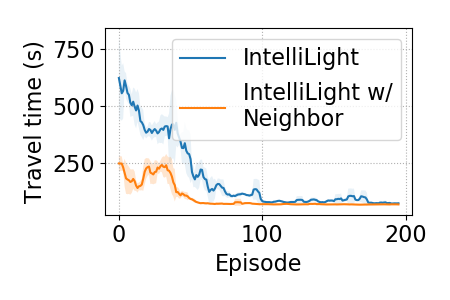
\includegraphics[width=0.4\textwidth]{figures/intro_0.png}\\
   \begin{tabular}[c]{@{}c@{}}(a) Performance w.r.t. reward\end{tabular} &
   \begin{tabular}[c]{@{}c@{}}(b) Convergence w.r.t. state\end{tabular} \\ 
   \end{tabular}
\label{fig:intro}
\caption{Performance of RL approaches is sensitive to reward and state. (a) A heuristic parameter tuning of reward function could result in different performances. (b) The method with a more complicated state (\LIT~\cite{ZXZF+19} w/ neighbor) has a longer learning time but does not necessarily converge to a better result. }
\label{fig:intro}
\vspace{-3mm}
\end{figure}

One major issue of current RL-based traffic signal control approaches is that the setting is often heuristic and lacks proper theoretical justification from transportation literature. This often results in highly sensitive performance w.r.t. the setting and leads to a long learning process. We elaborate on this issue by examining two fundamental elements in RL setting: reward and state.

First, various reward designs have been proposed in the literature. The reason is that travel time, the ultimate objective, is hard to optimize directly. Travel time is a long-term reward depending on a sequence of actions, thus the effect of one action can hardly be reflected in terms of travel time. People thus choose short-term rewards like queue length or delay to approximate the travel time~\cite{hua19survey}. So the reward function is often defined as a weighted sum of these terms~\cite{VaOl16,BPT14,ElAb10,ElAA13,wei2018intellilight}. However, as shown in Figure~\ref{fig:intro}(a), tuning the weights on these terms could lead to largely different results in terms of travel time. Some literature~\cite{ZZXW+19} discusses how to define the reward by connecting with the existing transportation method, but they only focus on controlling a single intersection. In this chapter, we focus on the multi-intersection control scenario. 

Second, existing RL methods have a trend of using more complicated state representation. Recent studies use visual images to describe the full traffic situation at the intersection~\cite{VaOl16,wei2018intellilight}, which results in the dimension of the state in the scale of thousands. In the single intersection scenario,~\cite{ZZXW+19} reveals that additional information is not always helpful. Similar conclusions can also be found in the multi-intersection scenario. As shown in Figure~\ref{fig:intro}(b), complicated state definitions increase the learning time and may not necessarily bring significant gain. Note that we are not claiming that additional information is always not helpful. The choice of the state depends on the reward setting. Based on the reward design of \LIT~\cite{ZZXW+19}, neighboring information is not necessary in the case we show in Figure~\ref{fig:intro}(b). The question is, could we justify theoretically how much information is enough in state definition in order to optimize the reward function?


\begin{figure}
    \centering
    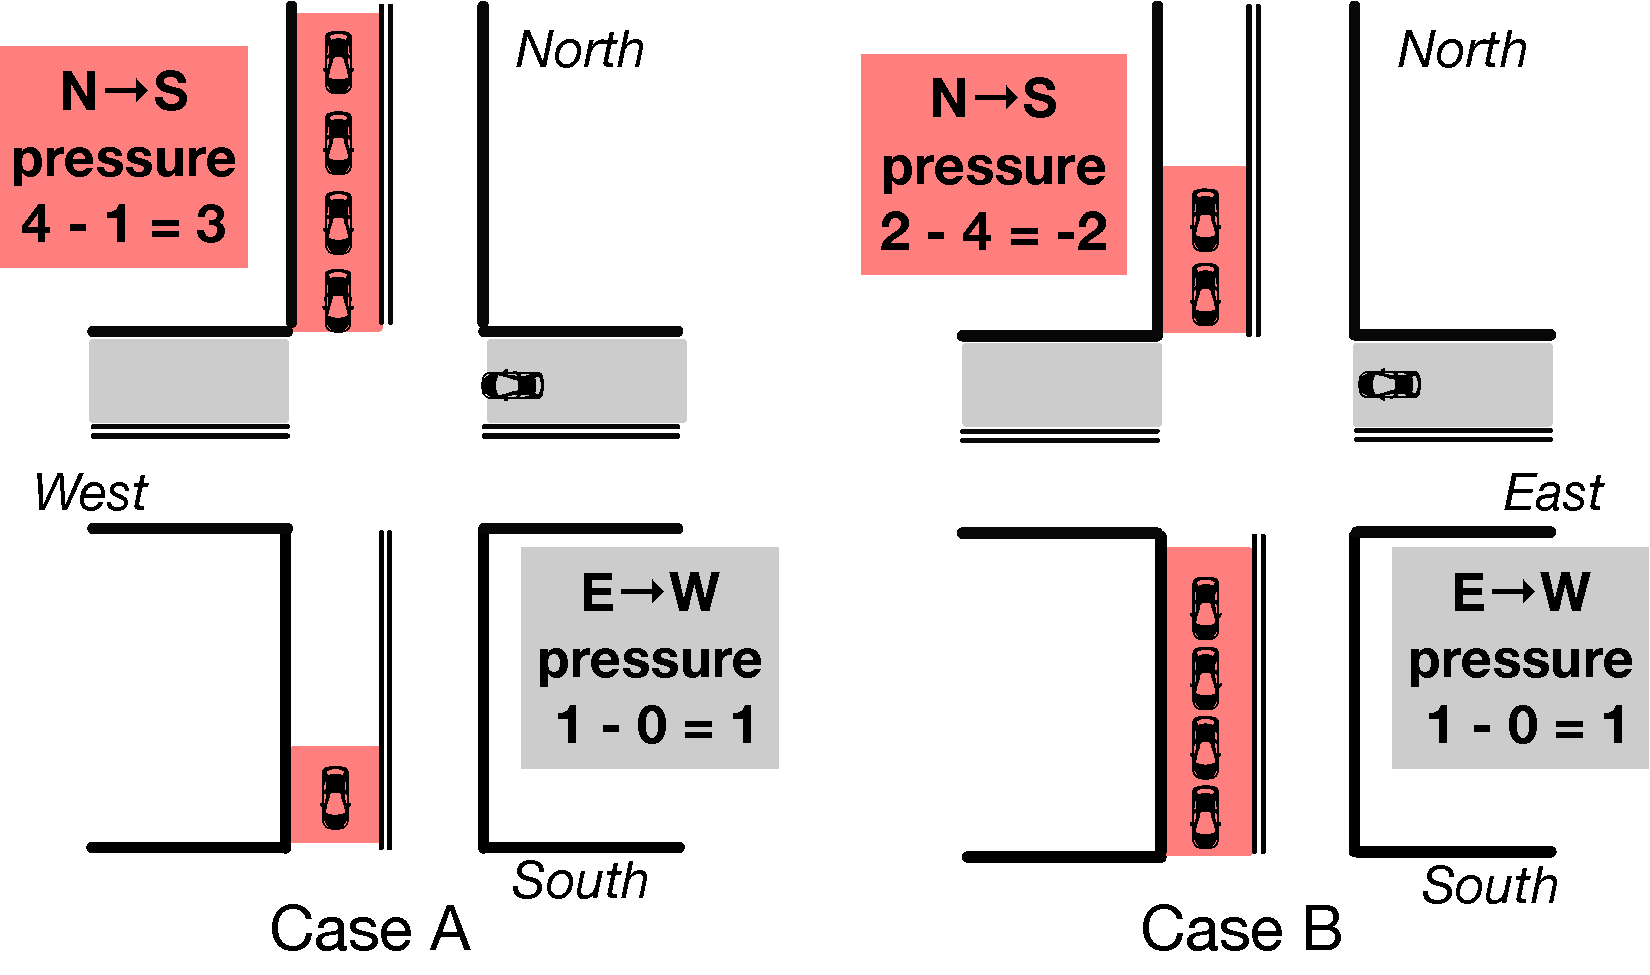
\includegraphics[width=0.8\textwidth]{figures/Maxpressure.pdf}
    \caption{Illustration of max pressure control in two cases. In Case A, green signal is set in the North$\rightarrow$South direction; in Case B, green signal is set in the East$\rightarrow$West direction.}
    \label{fig:pressure}
    \vspace{-2mm}
\end{figure}

The challenges we face in RL motivate us to look for support from transportation. In transportation literature, max pressure (MP) control is one of the state-of-the-arts in traffic signal control~\cite{MP13-adaptvie,MP13}. The key idea of MP is to minimize the ``pressure'' of an intersection, which can be loosely defined as the number of vehicles on incoming lanes minus the number of vehicles on outgoing lanes. Figure~\ref{fig:pressure} illustrates the concept of pressure. By setting the objective as minimizing the pressure of intersections, MP is proved to maximize the throughput of the whole road network\footnote{Maximizing throughput equals to minimizing travel time under certain conditions and minimizing travel time is the final goal for most traffic signal control problems.}. However, the solution of MP is greedy, which leads to locally optimal solutions. 

Our proposed solution is based on RL but theoretically grounded by MP method. The connection between RL and MP is that both approaches can essentially be framed as an optimization problem. In RL, long term reward is the objective for optimization and the solution is derived from trial-and-error search. In MP, the objective is to minimize pressure and the solution is derived from a greedy algorithm. Intuitively, if we set our reward function the same as the objective of MP, we can achieve the same result as MP. We first prove that under the assumption of no physical queue expansion, both our method and MP are maximizing throughput of the network. We further show that our method can relax the assumption on queue expansion and the conclusion still holds.

To further address the challenge on state design, we describe the system dynamics using the state features based on MP. MP provides evolution equations to formulate the state transition of the traffic as a Markov chain~\cite{MP13book}. In RL, the Markov decision process formally describes the dynamics of an environment. By including the variables from the evolution equation into state definition in RL, the state is a sufficient statistic for the system dynamics.

We conduct comprehensive experiments using both synthetic data and real data. We test our method in different traffic flow and network structure scenarios. We demonstrate the power of RL methods over traditional transportation approaches as RL optimizes the objective through trial and error. Our method also consistently outperforms state-of-the-art RL methods, which shows that theoretically supported reward design is necessary and the concise state design leads to an efficient learning process. We further discuss several interesting policies learned by our method to show that our method can achieve coordination along arterial.
\vspace{-3mm}

\section{Related Work}
\subparagraph{\textbf{Individual Traffic Signal Control.}}
Individual traffic signal control has been investigated extensively in the field of transportation, which tries to optimize the travel time or delay of vehicles~\cite{Gart83,Henr84,Boil06,SeHe97,Liang18}, assuming that vehicles are arriving and moving in a specific pattern. Recently, reinforcement learning based methods attempt to address this problem by directly learning from the data~\cite{Wier00,MaDH16}. Earlier work using tabular Q-learning~\cite{APK03,ElAb10} can only deal with discrete state representations. Recent work using deep RL~\cite{liLW16,VaOl16,wei2018intellilight,ZXZF+19,MSCH17,Casa17PG} can cope with more complex continuous state representation. ~\cite{ZZXW+19} noticed that it is not always true that the more complex the state definitions are, the better the performance will be. In~\cite{ZZXW+19}, they also investigated the proper reward design grounded by the individual intersection control method in transportation field. In this chapter, we are focusing on the multi-intersection scenario.

\subparagraph{\textbf{Conventional Multi-intersection Traffic Signal Control.}}
In conventional multi-intersection control, coordination can be achieved by setting a fixed offset (i.e., the time interval between the beginnings of green lights) among all intersections along an arterial~\cite{urbanik2015signal}. In fact, it is not an easy task, given traffic of opposite directions usually cannot be facilitated simultaneously. To solve this problem, some optimization-based methods~\cite{robertson1969transyt,little1981maxband} are developed to minimize vehicle travel time and/or the number of stops at multiple intersections. Instead of optimizing offsets, max pressure~\cite{MP13,MP13book} aims to maximize the throughput of the network so as to minimizing the travel time. However, these approaches still rely on assumptions to simplify the traffic condition and do not guarantee optimal results in the real world.

\subparagraph{\textbf{RL-based Multi-intersection Traffic Signal Control.}}
Since recent advances in RL improve the performance on isolated traffic signal control~\cite{wei2018intellilight,ZZXW+19}, efforts have been made to design strategies that control multiple intersections. \textit{One way} is to consider jointly modeling the action between learning agents with centralized optimization~\cite{KWBV08,VaOl16}. Since these methods~\cite{KWBV08,VaOl16} need to negotiate between the agents in the whole network, they are computationally expensive. \textit{Another way} is to use decentralized RL agents to control the traffic signals in the multi-intersection system~\cite{ElAA13,ALUK10,da2006adaptive}. Since each agent makes its own decision based on the information from itself and neighboring intersections without centralized decision, decentralized methods may be more scalable and practicable. By plugging new intersection controllers into the system, the decentralized systems are easy to scale. Our proposed method also follows this direction. 

We notice the recent trend to vary the definition of state and reward in RL for traffic signal control. Readers interested in the detailed comparison of the state and reward definitions can refer to~\cite{hua19survey}. We are the first RL method that is theoretically grounded by traditional transportation methods to coordinate the traffic signals along an arterial.


% !TEX root = main.tex
\section{Preliminaries}
\label{sec:preliminary}

\begin{definition}[Incoming lane and outgoing lane of an intersection]
An incoming lane for an intersection is a lane where the traffic enters the intersection. 
An outgoing lane for an intersection is a lane where the traffic leaves the intersection. 
We denote the set of incoming lanes and outgoing lanes of an intersection as $L_{in}$ and $L_{out}$ respectively.
\end{definition}
\vspace{-3mm}
\begin{definition}[Traffic movement]
A traffic movement is defined as the traffic traveling across an intersection from one incoming lane to an outgoing lane. We denote a traffic movement from lane $l$ to lane $m$ as $(l,m)$. 
% We call $m$ is the outgoing lane of $l$ and denote all the outgoing lanes of $l$ as $Out_l$.
\end{definition}
\vspace{-3mm}
\begin{definition}[Movement signal and phase]
A movement signal is defined on the traffic movement, with green signal indicating the corresponding movement is allowed and red signal indicating the movement is prohibited. We denote a movement signal as $a(l,m)$, where $a(l,m)=1$ indicates the green light is on for movement $(l,m)$, and $a(l,m)=0$ indicates the red light is on for movement $(l,m)$.
A phase is a combination of movement signals. We denote a phase as $p=\{(l,m)| a(l,m)=1\}$, where $l\in L_{in}$ and $m\in L_{out}$.
\end{definition}
In Figure~\ref{fig:preliminary}, there are twelve incoming lanes and twelve outgoing lanes in the intersection. Eight movement signals (red and green dots around the intersection) comprise \emph{four} phases to control the traffic movements for the intersection: \WEs (Going Straight from West and East), \SNs (Going Straight from South and North), \WEl (Turning Left from West and East), \SNl (Turning Left from South and North).  Specifically, \WEl allows two traffic movements. When phase \#2 is activated, the traffic from $l_E$ and $l_W$ is allowed to turn left to corresponding outgoing lanes.

\begin{definition}[Pressure of movement, pressure of intersection]
The pressure of a movement is defined as the difference of vehicle density between the incoming lane and the outgoing lane. The vehicle density of a lane is defined as $x(l)/x_{max}(l)$, where $x(l)$ is the number of vehicles on lane $l$, $x_{max}(l)$ is the maximum permissible vehicle number on $l$. We denote the pressure of movement $(l,m)$ as
\begin{equation}
\label{eq:pressure-movement}
w(l,m)=\frac{x(l)}{x_{max}(l)}-\frac{x(m)}{x_{max}(m)}
\end{equation}
If all the lanes have the same maximum capacity $x_{max}$, then $w(l,m)$ is simply indicating \textit{the difference between the incoming and outgoing number of vehicles}. 

The pressure of an intersection $i$ is defined as the sum of the absolute pressures over all traffic movements, denoted as:

\begin{equation}
    \label{eq:pressure}
    P_i = |\sum_{(l,m)\in i}w(l,m)\ |
\end{equation}

In Figure~\ref{fig:pressure}, the pressure of the intersection in Case A is $|3+1|=4$, whereas the pressure of intersection in Case B is $|-2+1|=1$. In general, the pressure $P_i$ indicates the degree of disequilibrium between the incoming and outgoing vehicle density. The larger $P_i$ is, the more unbalanced the distribution of vehicles is.
\end{definition}
\vspace{-3mm}
\begin{problem}[Multi-intersection traffic signal control]
In our problem, each intersection is controlled by an RL agent.  At each time step $t$, agent $i$ observes from the environment as its state $o^t_i$. Given the vehicle distribution and current traffic signal phase, the goal of the agent is to give the optimal action $a$ (i.e., which phase to set), so that the reward $r$ (i.e., the average travel time of all vehicles) can be maximized. %The multi-intersection traffic signal control problem can be formulated as a Markov game, see Section~\ref{sec:formulation} in Addendum for more details.
\end{problem}

%Figure~\ref{fig:pressure} shows two cases indicating different pressures. There are only two phases in both cases: One phase activates the traffic movement along arterial (North to South), the other activates the movement along side road (East to West). The pressure for traffic movement from North to South in Case A is the larger than Case B, indicating the green light for North to South movement in Case A is more demanded.


\begin{figure}
    \centering
    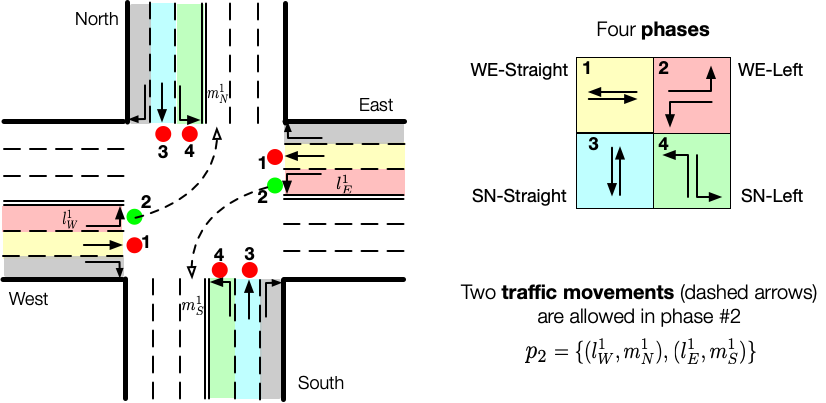
\includegraphics[width=0.8\textwidth]{figures/phase.png}
    \caption{Phase and traffic movements in traffic signal control problem. Phase \#2 is set in the example.}
    \label{fig:preliminary}
    % \vspace{-2mm}
\end{figure}

\vspace{-2mm}
% !TEX root = main.tex
\section{Method}

\subsection{Agent Design}
\label{sec:formulation}

First, we introduce the state, action and reward design for an agent that controls an intersection.
\begin{itemize}[wide,noitemsep,topsep=0pt]
    \item \textbf{State (Observation)}. Our state is defined for one intersection, which equals to the definition of observation in multi-agent RL. It includes the current phase $p$, the number of vehicles on each outgoing lane $x(m)$ ($m\in L_{out}$), and the number of vehicles on each segment of every incoming lane $x(l)_k$ ($l\in L_{in}$, $k=1\dots K$). In this chapter, each lane is evenly divided into 3 segments $(K=3)$, and we denote the segment on lane $l$ nearest to the intersection as the first segment $x(l)_1$.
    \item \textbf{Action}. At time $t$, each agent chooses a phase $p$ as its action $a_t$ from action set $\pmb{A}$, indicating the traffic signal should be set to phase $p$. In this chapter, each agent has four permissible actions, correspondingly four phases in Figure~\ref{fig:preliminary}. Each action candidate $a_{i}$ is represented as a one-hot vector. Note that in the real world the signal phases may organize in a cyclic way, while our action makes the traffic signal plan more flexible. Also, there may be different number of phases in the real world and four phases is not a must.
    \item \textbf{Reward}. We define the reward $r_i$ as
        \begin{equation}
            \label{eq:reward-detail}
            r_i  = - P_i,
        \end{equation}
    where $P_i$ is the  \textit{\textbf{pressure}} of intersection $i$, as defined in Equation~\eqref{eq:pressure}.
    
    Intuitively, the pressure $P_i$ indicates the degree of disequilibrium between vehicle density on the incoming and outgoing lanes. By minimizing $P_i$, the vehicles within the system can be evenly distributed. Then the green light is effectively utilized so that the throughput is optimized.
    
    % If we regard all the intersections have the same maximum capacity $x_{max}$ and $x(l,m)^{down}=\sum_{p\in Out_m}{r(m,p)\cdot x(m,p)}$ as the downstream number of vehicles and $x(l,m)$ as the incoming number of vehicles, then 
    % \begin{equation}
    % w(l,m)= x(l,m)-x^{down}(l,m)
    % \end{equation}
    % is simply \textit{the difference between the incoming and downstream number of vehicles}. If the vehicles are not allowed to change their lanes, then $|Out_m|=1$ and $r(m,p)=1$, we have $w(l,m)= x(l,m)-x(m,p)$, which is simply the difference of number of vehicles between the incoming and downstream lane.
\end{itemize}

\vspace{-1mm}
\subsection{Learning Process}

% At each time step $t$, each agent $i$ aim to find the action $a_i$ that lead to the maximum total discounted future reward:
% \begin{equation}
%     G^t_i=\Sigma_{k=t}^\infty\gamma^{k-t}r_i^t
% \end{equation}
% from time step $t$ onwards, where the discount factor $\gamma \in [0, 1]$ controls the importance of immediate rewards versus future rewards. 

% The policy $\pi$ of agent $i$ has a corresponding action-value function that gives the expected return conditioned on the observation $o$ and action $a$, when acting according to that policy:

% \begin{equation}
% Q^\pi_i(o,a) = \mathbb{E}[G^t_i|o_t=o,a_t=a,\pi]
% \end{equation}

% The optimal policy $\pi^*$ can be found by iteratively improving an estimate of the optimal action-value function
% \begin{equation}
% \label{eq:q_max}
% Q^*_i(o, a) := \max_\pi Q^\pi_i(o, a)
% \end{equation}
% using sample-based updates. Once $Q^*_i$
% is sufficiently approximated, acting greedy with respect to it yields the optimal policy.

% The Q-value function is estimated using a function approximator with weight vector $\theta: Q_i(o, a; \theta)$. 

In this chapter, we adopt Deep Q-Network (DQN) as function approximator to estimate the Q-value function. To stabilize the training process, we maintain an experience replay memory as described in~\cite{MKSR+15} by adding the new data samples in and removing the old samples occasionally. Periodically, the agent will take samples from the memory and use them to update the network.
% \begin{figure}[h!]
% \includegraphics[width = 250pt]{figures/qnetwork.png}
% \caption{Deep Q-network}
% \label{fig:q-network}
% \end{figure}


\section{Justification of RL agent}
To theoretically support the efficacy of our proposed method, we justify our reward and state design by showing that, in a simplified transportation system, the states we use can fully describe the system dynamics, and using Equation~\eqref{eq:reward-detail} as reward function in RL is equivalent to optimizing travel time as in the transportation methods. Some important notation is summarized in Table~\ref{tab:notations}.
\vspace{-3mm}

\begin{table}[htb]
\centering
  \caption{Summary of notation.}
  \label{tab:notations}
  \begin{tabular}{cl}
    \toprule
    Notation&Meaning\\
    \midrule
    $L_{in}$ & set of incoming lanes for an intersection \\
    $L_{out}$ & set of outgoing lanes for an intersection \\
	$(l,m)$ &\begin{tabular}[c]{@{}l@{}}a traffic movement from lane  $l$ to $m$
	\end{tabular} \\
    $x(l,m)$ & number of vehicles leaving $l$ and entering $m$\\
    $x(l)$ & number of vehicles on lane $l$\\
    $x(l)_k$ & number of vehicles on $k$-th segment of $l$\\
    $x_{max}(m)$ & maximum permissible vehicle number on lane $m$ \\
    $r(l,m)$ & turning ratio of traffic movements from $l$ to $m$\\
    $c(l,m)$ & discharging rate of movement $(l,m)$\\
    %$C(l,m)$ & saturation flow of phase $(l,m)$, vehicles per timestep\\
    $a(l,m)$ & \begin{tabular}[c]{@{}l@{}} 1 if the green light is on for movement $(l,m)$,\\ 0 otherwise
	\end{tabular} \\
	%$P_i$ & pressure on intersection $n$\\
    % $L$ & length of a road segment\\
  \bottomrule
\end{tabular}
\vspace{-3mm}
\end{table}

\subsection{Justification for State Design}

\subsubsection{General description of traffic movement process as a Markov chain}

Consider the arterial scenario described in Example~\ref{eg:inter}.
\begin{figure}[h!]
\centering
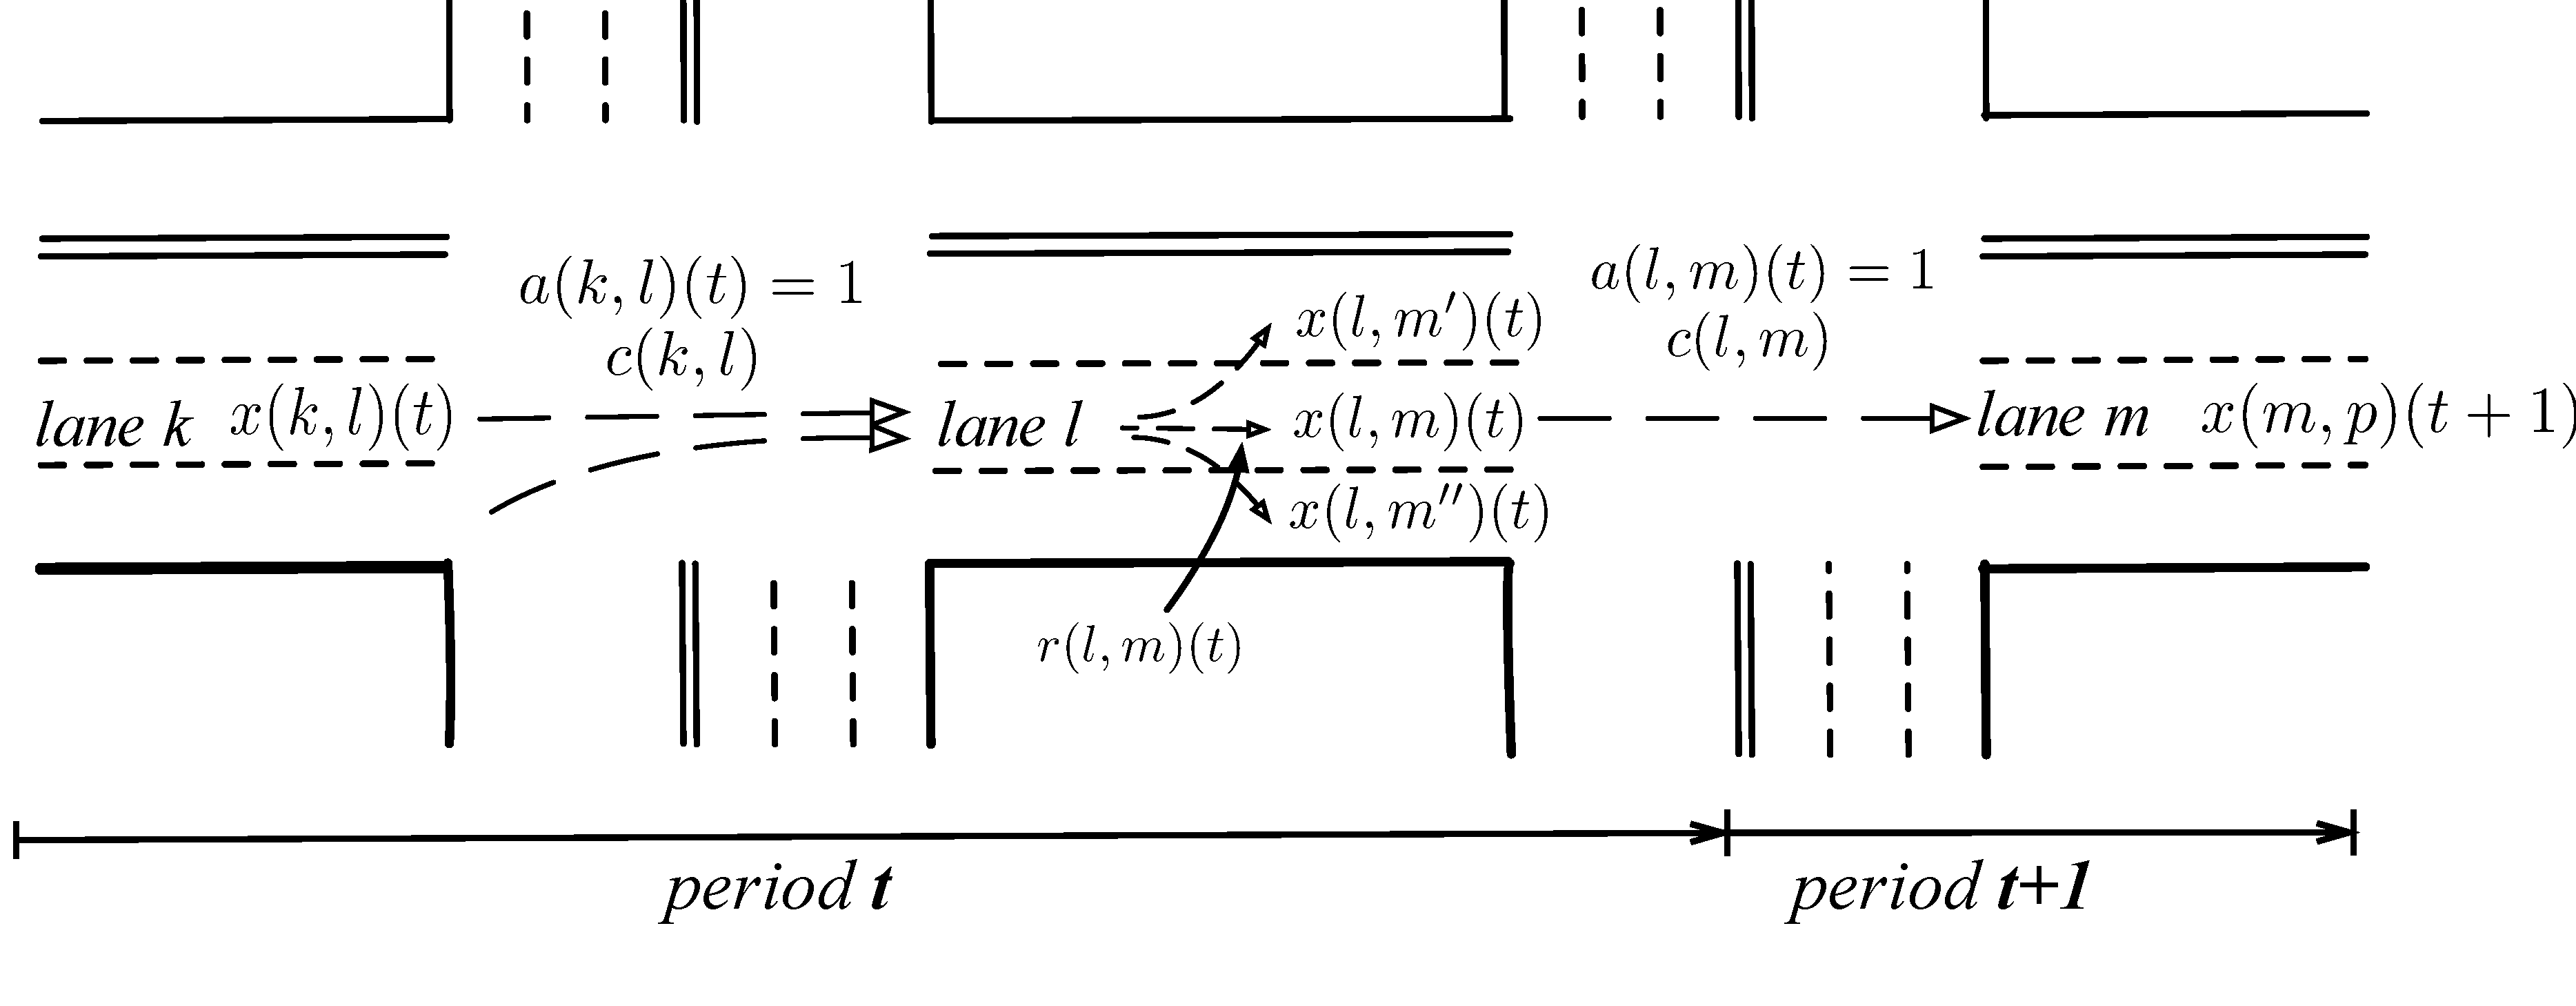
\includegraphics[width = 5.0in]{figures/SFM.pdf}
\caption{The transition of traffic movements.}
\label{fig:SFM}
\vspace{-3mm}
\end{figure}

\begin{example}
\label{eg:inter}
Figure~\ref{fig:SFM} associates a distinct traffic movement with each incoming lane $l\in L_{in}$ and each $m\in Out_l$, where $Out_l$ is the set of lanes output from lane $l$. 
Follow the notation from~\cite{MP13book}, let $x(l,m)(t)$ be the associated number of vehicles at beginning of period $t$, $X(t) = \{x(l,m)(t)\}$ is the $state$ of the movement network, which we regard as states $o^t$ in accordance with Section~\ref{sec:formulation}. There are two variables which are considered independent of $X(t)$: 
\begin{itemize}[wide,noitemsep,topsep=0pt]
    \item Turning ratio $r(l,m)$: $r(l,m)$ is an i.i.d. random variable indicating the proportion of vehicles entering $m$ from $l$ to the total vehicles on $l$. 
    
    \item Discharging rate $c(l,m)$: For each $(l,m)$, the queue discharging rate $c(l,m)$ is a non-negative, bounded, i.i.d. random variable,  i.e., $c(l,m)\leq C(l,m)$, where $C(l,m)$ is the saturation flow rate.
    
    % \item Demand $d(l,m)(t)$:  For each entry lane $l$, $d(l,m)$ are also non-negative bounded iid random variables. 
\end{itemize}

At the end of each period $t$, an action $A^t=\{(l,m)|a^t(l,m)\}$ must be selected from the action set $\pmb{A}^t$ as a function of $X^t$ for use in period $(t+1)$, indicating the agent will give green light for movements from $l$ to $m$, see the bottom of Figure~\ref{fig:SFM}. 

\end{example}

 The evolution equations of $X(t)$ are developed in~\cite{MP13}. For each $(l,m)$ and $t$, the evolution of $x(l,m)$ consists of receiving and discharging, and is captured by the following equation:
\begin{equation}
\begin{split}
\label{eq:queue-process}
      & x(l,m)(t+1) \\
    = &\ x(l,m)(t) + \ \underbrace{ \Sigma_{k\in In_l} min[c(k,l)\cdot a(k,l)(t),\ x(k,l)(t)]\cdot r(l,m)}_{receiving\ vehicles}\\
    - &\ \underbrace{ min\{c(l,m)\cdot a(l,m)(t),\ x(l,m)(t)\}\cdot \mathbf{1}(x(m)\le x_{max}(m))}_{discharging\ vehicles},\\
\end{split}
\end{equation}
where $In_l$ represents the set of lanes input to $l$. For the second term in Equation~\eqref{eq:queue-process}, when $l$ is the receiving lane, up to $x(k,l)$ vehicles will move from $k$ if $a(k,l)(t)=1$ and they will join $(l,m)$ if $r(l,m)=1$
For the third term in Equation~\eqref{eq:queue-process}, when traffic movement $(l,m)$ is actuated, i.e., $a(l,m)(t)=1$, up to $x(l,m)$ vehicles will leave $l$ and be routed to $m$ if there is no blockage on lane $m$, i.e., $x(m)\leq x_{max}(m)$, where $x_{max}(m)$ is the maximum permissible vehicle number on lane $m$. 

\nop{
    \begin{equation}
    x(l,m)(t+1) = x(l,m)(t)+\delta(l,m)(t)
    \end{equation}
    where,
    \begin{align*}
    g_l(t) = min\{c(l,m)(t+1)\cdot a(l,m)(t),\ x(l,m)(t)\}\cdot \mathbf{1}(x(m)\le x_{max}(m)), \\ l\in\mathcal{L}, m\in Out_l
    \end{align*}
    
    \begin{align*}
    f_l(t) = \sum_k min[c(k,l)(t+1)\cdot a(k,l)(t),\ x(k,l)]\cdot r(l,m)(t+1)\\
     l\in \mathcal{L}, k\in In_l\\
    \end{align*}
}

% For entry lanes of the system which have exogenous arrivals and no input lanes, the update equation is different: Equation~\ref{eq:queue-process} is modified to:
% \begin{equation}
% \begin{split}
% \label{eq:queue-process-entry}
%       & x(l,m)(t+1) \\
%     = & x(l,m)(t) +  d(l,m)(t)\\
%     - & min\{c(l,m)\cdot a(l,m)(t),\ x(l,m)(t)\}\cdot \mathbf{1}(x(m)\le x_{max}(m)) \\
% \end{split}
% \end{equation}

%In~\cite{MP13}, the time frame $t\rightarrow t+1$ is assumed to be the lane travel time, which has two disadvantages: (1) It assumes all the lane travel time is the same no matter the lane length. (2) It is resource consuming to take the traffic conditions $x(k,l)$ of nearby intersections. 

Suppose the initial state $X(1)={x(l,m)(1)}$ is a bounded random variable. Since $A(t)={a(l,m)(t)}$ is a function of the current state $X(t)$, and $c(l,m)$ and $r(l,m)$ are all independent of $X(1),...,X(t)$, the process $X(t)$ is a \textit{\textbf{Markov chain}}. The transition probabilities of the chain depend on the control policy.


\subsubsection{Specification with proposed state definition}
We can modify the traffic movement equation from lane-level to segment-level. We denote $x(l)_1$ as the number of vehicles on the segment $l_1$ closest to the intersection and $x(l)_2$ as the number of vehicles on the second closest segment, which is connected with $l_1$. Assume the vehicles change lanes for routing by the time it enters the lane $l$, i.e., $x(l,m)=x(l)$, and all vehicles on $l_{i+1}$ enter next segment $l_{i}$ during time $t$, then the movement process on the segment closest to the intersection can be written as:
\begin{equation}
\begin{split}
\label{eq:queue-process-segnment}
      & x(l)_1(t+1) = \ x(l)_1(t) + \ x(l)_2(t)\\
    - &\ min\{c(l,m)\cdot a(l,m)(t),\ x(l)_1(t)\}\cdot \mathbf{1}(x(m)\le x_{max}(m)). \\
\end{split}
\end{equation}
Equations for other segments can be derived in a similar way. 
 
With the lane and segment movement evolution equations described above, the evolution of an individual intersection could be obtained, which is a combination of the equations of all the lanes involved. For a single intersection $i$, $c(l,m)$ is a constant physical feature of each movement, whereas $x(l)_1$, $x(l)_2$, and $x(m)$ are provided to the RL agent in our state definition. Hence, our state definition can fully describe the dynamics of the system.


\subsection{Justification for Reward Design}
\subsubsection{Stabilization on traffic movements with proposed reward.}
Inspired by~\cite{MP13}, we first relax its assumption on physical queue expansion in the arterial. Then the goal of our RL agents is proven to stabilize the queue length, thus maximizes the system throughput and minimizes the travel time of vehicles.

%\theoremstyle{Definition}

\begin{definition}[Movement process stability] 
The movement process $X(t) = \{x(l, m)(t)\}$ is stable in the mean (and $u$ is a stabilizing control policy) if for
some $M<\infty$, the following holds:
\begin{equation}
\label{eq:stability}
    \sum_{t=1}^{T}\sum_{(l,m)}E[x(l,m)(t)]<M,\quad\forall T
\end{equation}
where $E$ denotes expectation. Movement stability in the mean implies that the chain is positive recurrent and has a unique steady-state probability distribution for all $T$. 
\end{definition}


\begin{definition}[Max-pressure control policy~\cite{MP13}] 
\label{def:maxpressure}
At each period $t$, the agent selects the action with maximum pressure at every state $X$: $
\tilde{A}^*(X) = \arg\max_{\tilde{A}\in \pmb{A}}\theta(\tilde{A}, X)$, where the pressure of $\tilde{A}$ is defined as
$$\theta(\tilde{A},X) = \sum_{(l,m):a(l,m)=1} \tilde{w}(l,m),$$
and $\tilde{w}(l,m) = x(l)- x(m)$ is the pressure of each movement. 
In this chapter, we use the tilde symbol for max-pressure policy, i.e., $\tilde{A}$, in order to differentiate it from a RL policy.
% \begin{equation}
% \label{eq:mp-pressure}
% \theta(\tilde{A},X) = \sum_{l,m:a(l,m)=1}c(l,m)\cdot \tilde{w}(l,m)(X)
% \end{equation}
\end{definition}

\begin{theorem}
\label{theo:stable} Without considering the physical queue expansion\footnote{``Without physical queue expansion'' means the vehicles will be considered to have no physical length in a queue.}, action $\tilde{A}^*$ selected by max-pressure control policy and action $A^*$ selected by our RL policy are both stabilizing the system, whenever the average demand is admissible\footnote{Intuitively, an admissible demand means the traffic demand can be accommodated by traffic signal control strategies, not including situations like long-lasting over-saturated traffic that requires perimeter control to stop traffic from getting in the system.}.
\end{theorem}

\begin{proof}For max-pressure control policy, Theorem 1 in~\cite{MP13} shows that given a time period $t=1,\ldots,T$ there exists $m<\infty$ and $\epsilon>0$ such that under $\tilde{A}^*$:
% \begin{equation}
% \label{eq:stability-proof}
% \epsilon\cdot\frac{1}{T}\sum_{t=1}^TE[X(t)]\leq m + \frac{1}{T}\cdot E[X(1)]^2
% \end{equation}
$\epsilon\cdot\frac{1}{T}\sum_{t=1}^TE[X(t)]\leq m + \frac{1}{T}\cdot E[X(1)]^2
$, 
where $X(1)$ denotes the state when $t=1$. 

For an optimal RL control policy, the agent selects the action $A$ with optimal $Q (A,X)$ at every state $X$:
\begin{equation}
\label{eq:q_max}
A^*(X) = \arg\max_{A\in \pmb{A}}Q(A, X).
\end{equation}
where $Q_t(A,X)= E[r_{t+1}+\gamma r_{t+2}+\dots | A, X]$ denotes the maximum total reward at state $X$ by taking $A$ at time $t$(in Equation~\eqref{eq:q_max}, we neglect time $t$ for simplicity).
The difference between the pressure definition in RL reward and max-pressure is that our RL agent uses the weighted pressure considering maximum permissible vehicle number $x_{max}$ in Equation~\eqref{eq:pressure-movement}. If we assume the lanes are in the same lenth $x_{max}(l)$, the stability result still holds for the normalized $x(l)$.
\end{proof}

\begin{theorem}
\label{theo:stable} Considering the physical queue expansion in the arterial environment, action $A^*$ selected by our RL policy is also stabilizing the movement.
\end{theorem}


\begin{figure*}[t!]
  \centering
    %   \begin{tabular}{ccc}
    %     %   \includegraphics[width=0.25\textwidth]{figures/case_beaver.png} &
    %     %   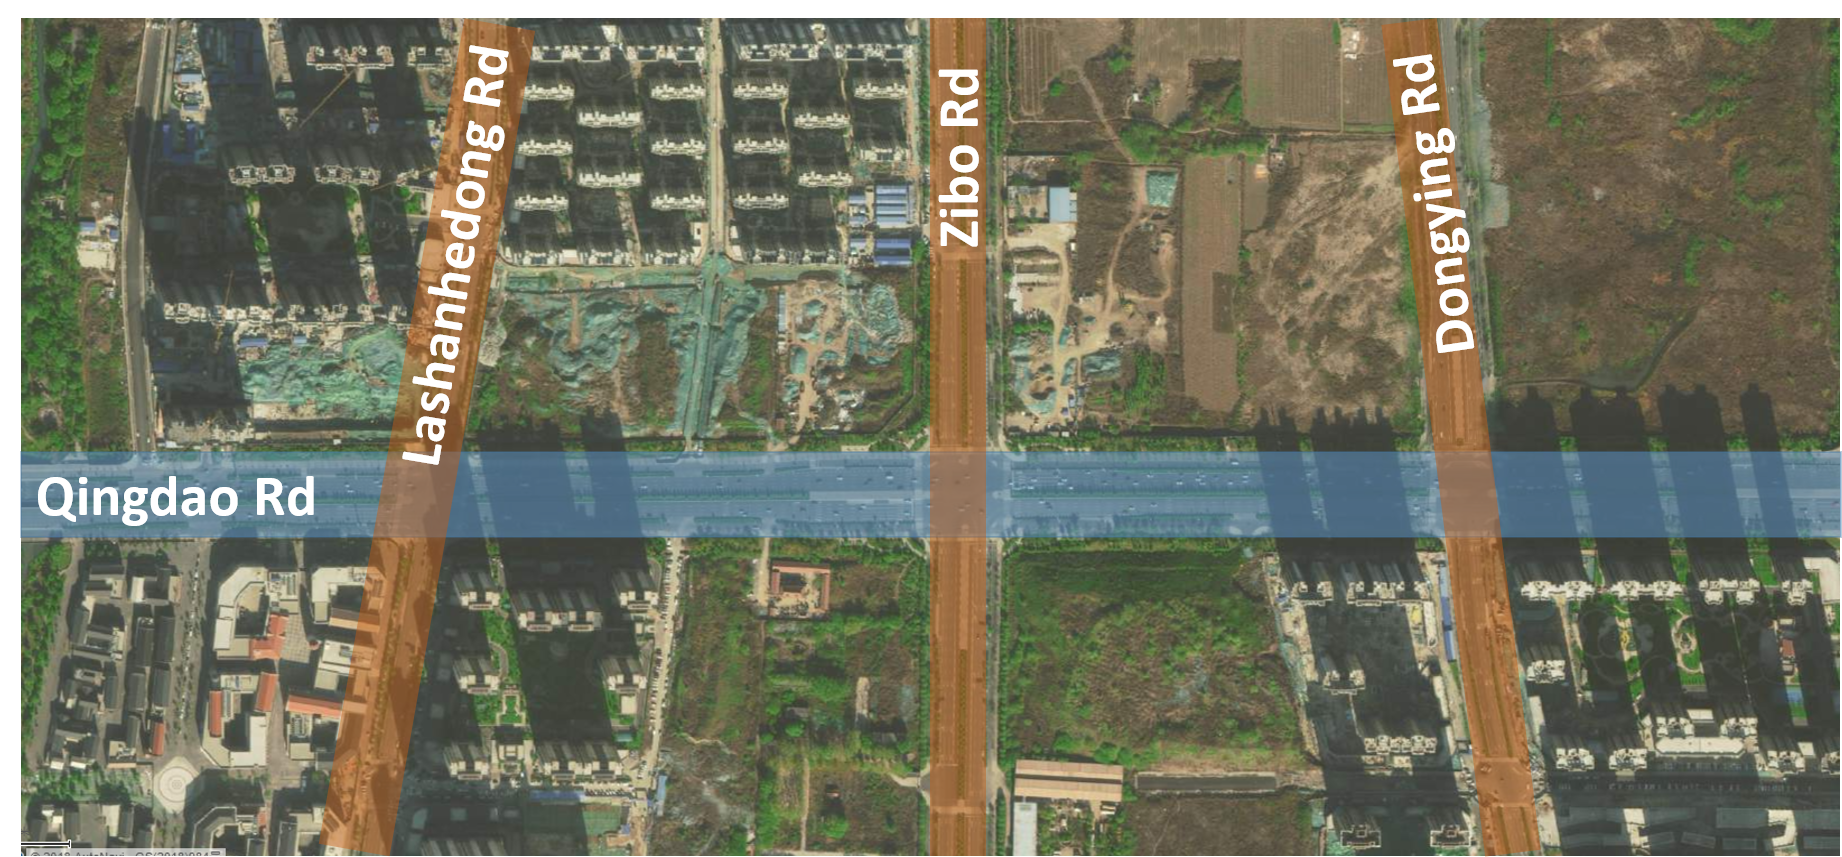
\includegraphics[width=0.22\textwidth]{figures/case_intersection_note.png}&
    %     %   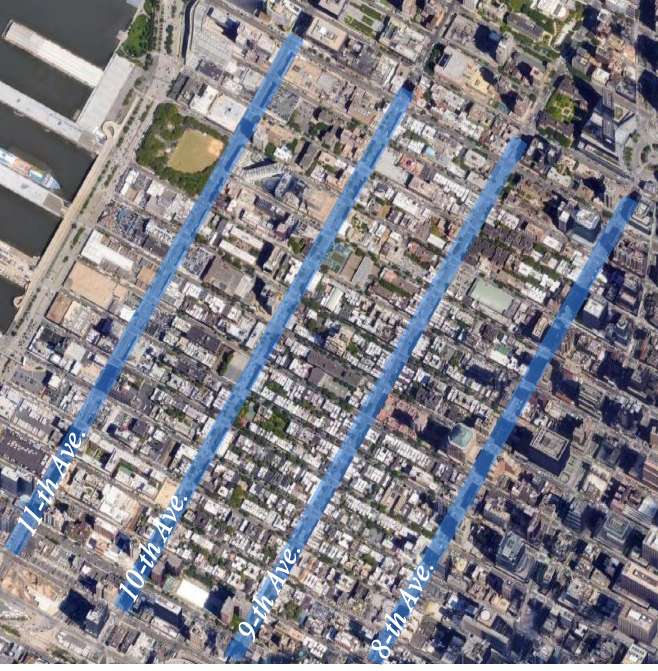
\includegraphics[width=0.42\textwidth]{figures/case_ny.png} \\
    %     %   \begin{tabular}[c]{@{}c@{}}(a) Beaver Avenue in State College, Pennsylvania, USA: \\a 5-intersection arterial with unidirectional traffic on the arterial\\ and bidirectional traffic on the side streets.\end{tabular}&
    %     %   \begin{tabular}[c]{@{}c@{}}(b) Qingdao Road in Jinan, China:\\ a 3-intersection arterial with bidirectional traffic \\on both the arterial and the side streets.\end{tabular}&
    %     %   \begin{tabular}[c]{@{}c@{}}(c) 8-th, 9-th, 10-th and 11-th Avenue in New York City, USA:\\ 16-intersection arterials with uni-directional traffic \\on both the arterial and the side streets.\end{tabular}\\
    %     %   \end{tabular}
    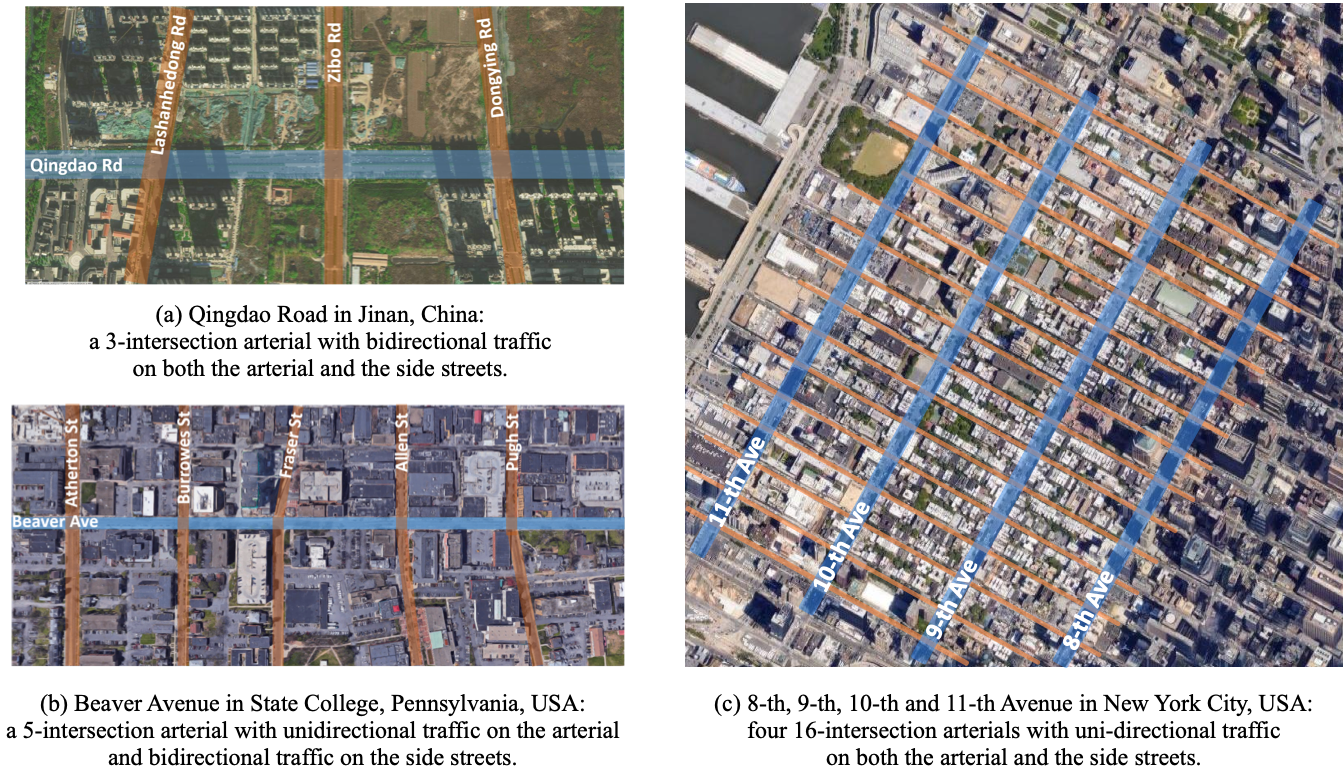
\includegraphics[width=1.0\textwidth]{figures/case_arterial.png}
     \caption{Real-world arterial network for the experiment.}
    \label{fig:real-intersection}
\end{figure*}

Different from~\cite{MP13}, we now establish the proof of Theorem~\ref{theo:stable}, which removes the assumption of no physical queue expansion in the arterial environment. In the arterial environment:
\begin{itemize}[wide,noitemsep,topsep=0pt]
    \item The maximum permissible vehicle number $x_{max}$ on side street lane $m^{side}$ is assumed to be infinite, hence the second term in Equation~\eqref{eq:pressure-movement} is zero. Thus we have $w(l,m^{side})=\frac{x(l)}{x_{max}(l)}>0$.
    \item When the outgoing lane $m^{main}$ along the arterial is saturated, the second term in Equation~\eqref{eq:pressure-movement} is approximately 1 because of the queue expansion. Thus $w(l,m^{main})\approx \frac{x(l)}{x_{max}(l)} -1 < 0$. 
\end{itemize}

This means when we consider the physical queue expansion in the arterial, $w(l,m^{side}) > w(l,m^{main})$, the control policy will restrict the queue spillback since it prohibits more vehicles to rush into the downstream intersection and block the movements of vehicles in other phases. Accordingly, $M$ in Equation~\eqref{eq:stability} can now be set to $M\leq \sum_{t=1}^{T}\sum_{(l,m)} x_{max}(m)$. 

\subsubsection{Connection to throughput maximization and travel time minimization.} Given that the traffic movement process of each intersection is stable, the system is accordingly stable. In an arterial environment without U-turn, vehicles that move from lane $m$ to $l$ would not move from $l$ to $m$ again, i.e.,  between $x(m,l)$ and $x(l,m)$ only one of them can exist under arterial network. Then the actions that RL agents take will not form gridlock or block the network, thus can efficiently utilize the green time. Within the given time period $T$, our RL agent can provide the maximum throughput, thus minimize the travel time of all vehicles within the system.

% !TEX root = main.tex

% \begin{figure*}[t!]
%   \centering
%   \begin{tabular}{cc}
%   \includegraphics[width=0.45\textwidth]{figures/case_beaver.png} &
%   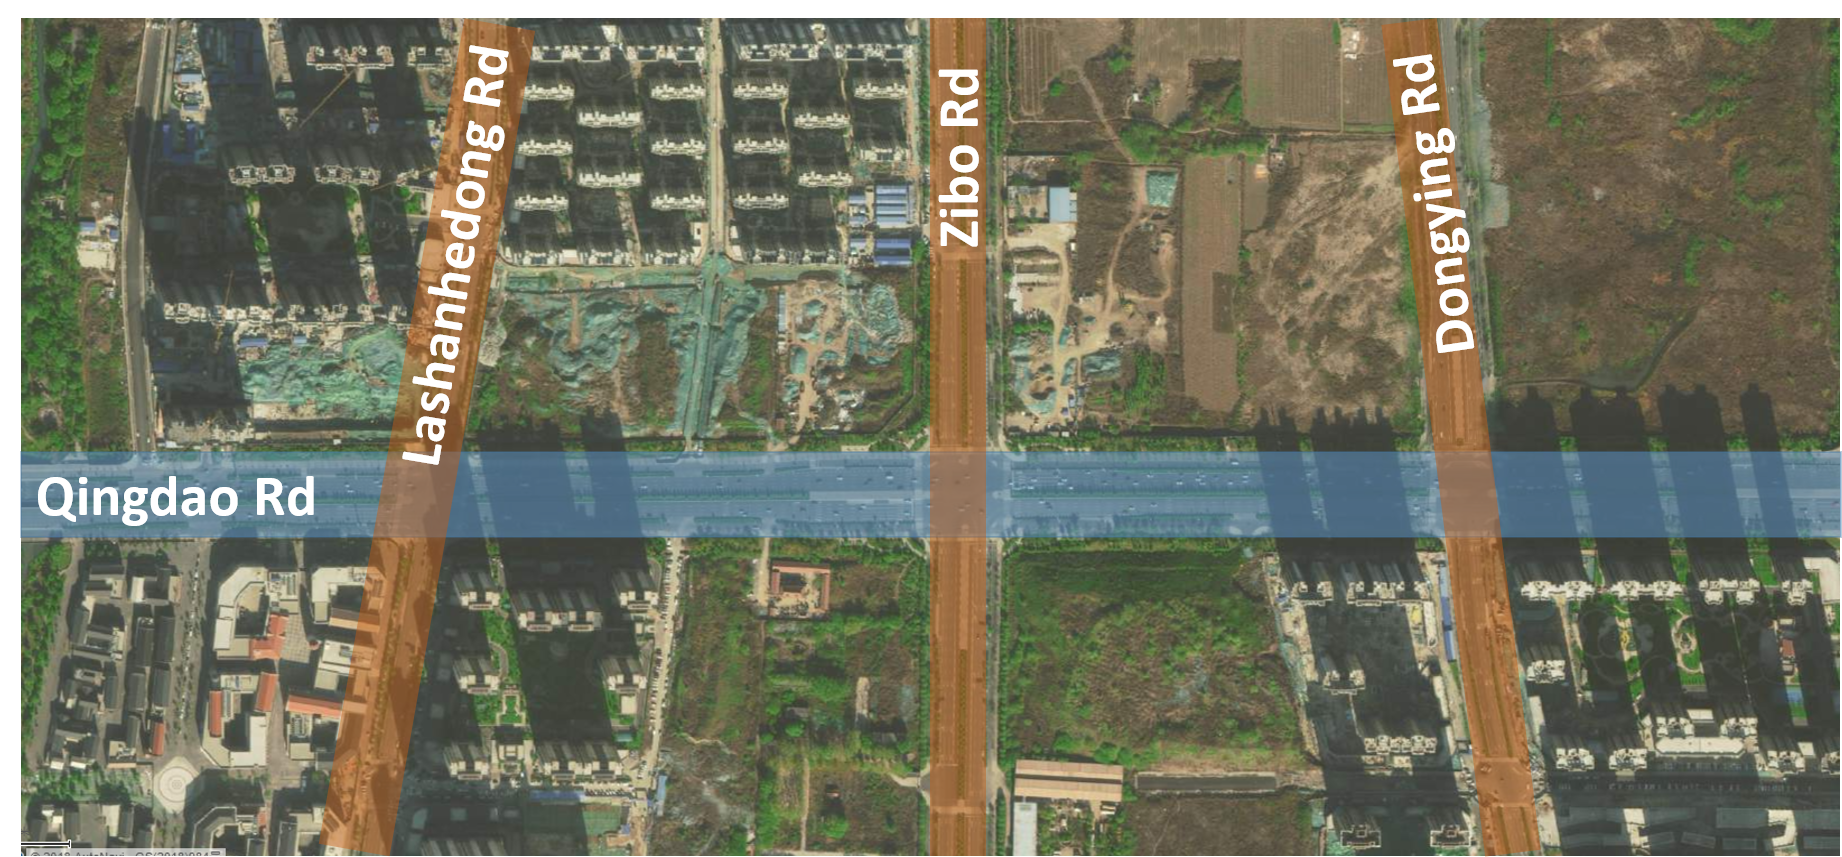
\includegraphics[width=0.42\textwidth]{figures/case_intersection_note.png} \\
%   \begin{tabular}[c]{@{}c@{}}(a) Beaver Avenue in State College, Pennsylvania, USA: \\a 5-intersection arterial with unidirectional traffic on the arterial\\ and bidirectional traffic on the side streets.\end{tabular}&
%   \begin{tabular}[c]{@{}c@{}}(b) Qingdao Road in Jinan, China:\\ a 3-intersection arterial with bidirectional traffic \\on both the arterial and the side streets.\end{tabular}\\
%   \end{tabular}
   
%      \caption{Real-world arterials for experiment.}
%     \label{fig:real-intersection}
% \end{figure*}

\section{Experiment}
We conduct experiments on CityFlow\footnote{http://cityflow-project.github.io}, an open-source traffic simulator that supports large-scale traffic signal control~\cite{huichu19}. After the traffic data being fed into the simulator, a vehicle moves towards its destination according to the setting of the environment. The simulator provides the state to the signal control method and executes the traffic signal actions from the control method.\footnote{Codes, public datasets and their preprocessing and
statistical details can be found at: https://github.com/wingsweihua/presslight. \\More datasets can be found at: http://traffic-signal-control.github.io}

\subsection{Dataset Description}
Both synthetic and real-world traffic flow data are used in our experiments. In a traffic dataset, each vehicle is described as $(o, t, d)$, where $o$ is  origin location, $t$ is  time, and $d$ is  destination location. Locations $o$ and $d$ are both locations on the road network. Traffic data is taken as input for the simulator. All the data contains bi-directional and dynamic flows with turning traffic. 

% \subsubsection{Road network data}
% Without losing generality, following road networks are tested in our experiment:
% \begin{itemize}[wide,noitemsep,topsep=0pt]
% \item Arterials with different numbers (6, 10, 20) of homogeneous intersections. 
% %, see Figure~\ref{fig:Traffic-direc-pattern}. 
% Each lane is five meters wide and 300 meters long. We use this environment to show the effectiveness of our method under different kinds of traffic flows. 
% % \begin{figure}[htb]
% %   \centering
% % 	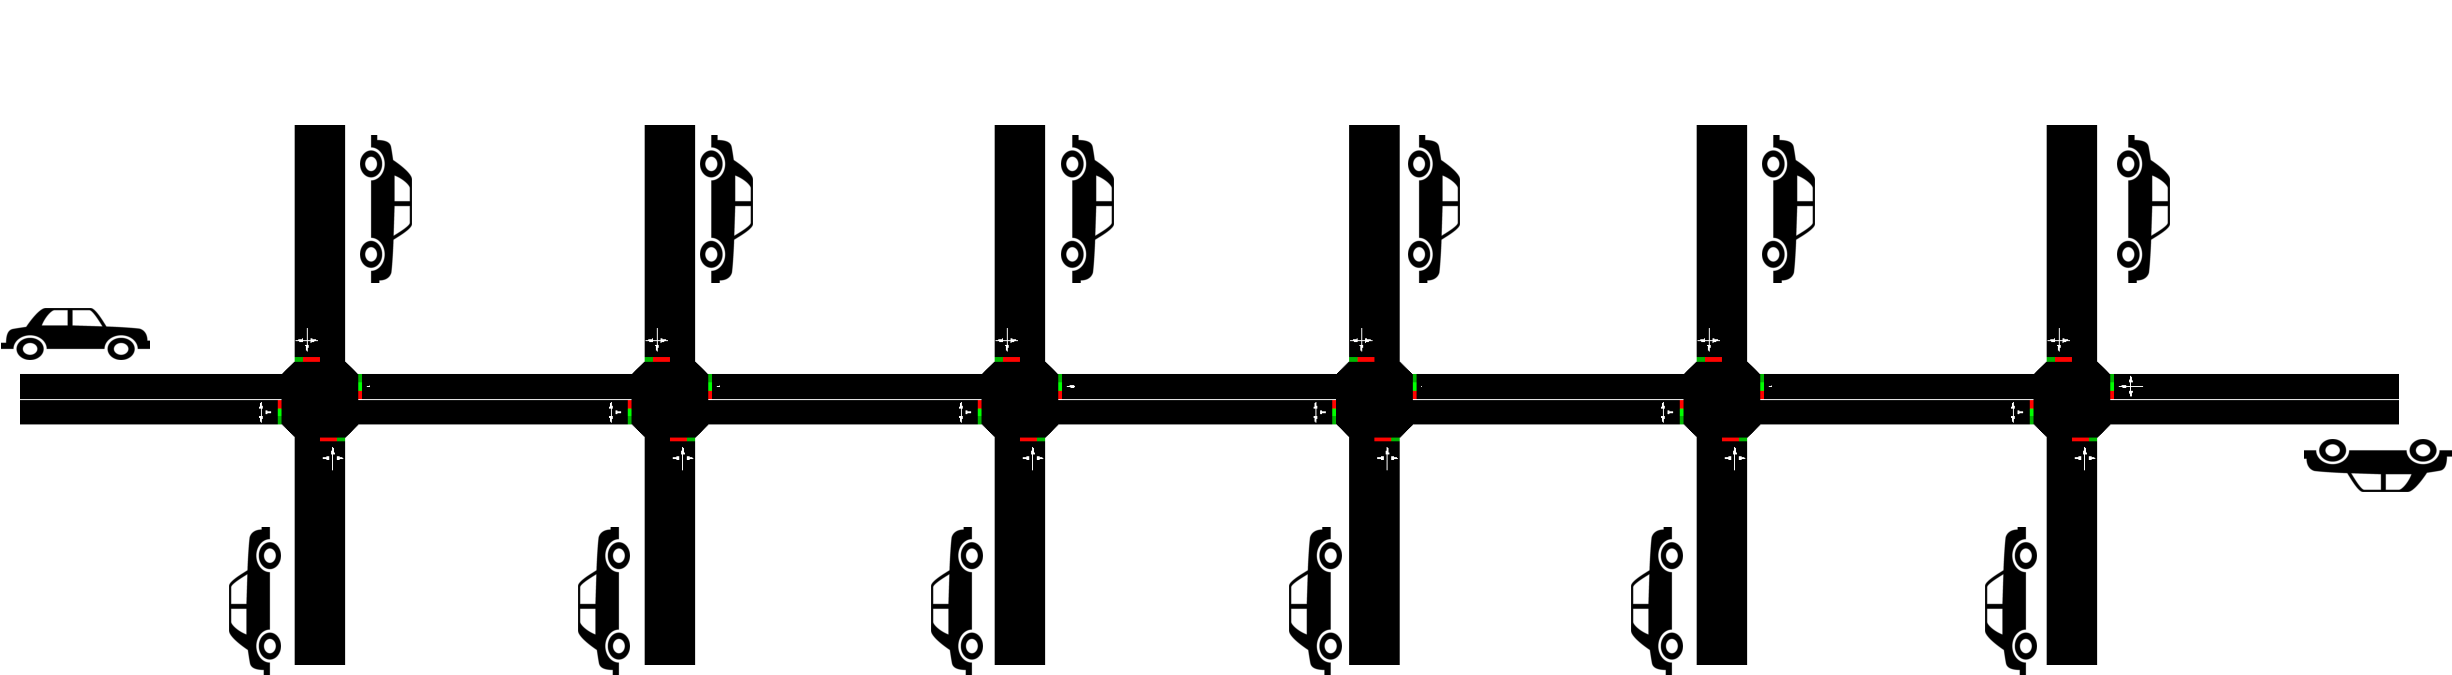
\includegraphics[width=0.48\textwidth]{figures/arterial_6.pdf}
% %      \caption{Bidirectional traffic on an arterial with 6 intersections.}   
% %     \label{fig:Traffic-direc-pattern}
% % \end{figure}
% % \item Arterial with 6 homogeneous intersections. This part of experiments are conducted on an arterial with four-leg intersections, see Figure~\ref{fig:Traffic-direc-pattern}. Each lane is 5 meters wide and 300 meters long. We use this environment to show the effectiveness of our method under different kinds of traffic flows. 
% \item Three-intersection arterials with different length of lanes (300-meters long and 150-meters long), and different legs (3 legs and 4 legs), as illustrated in~\ref{fig:heter_inter}. We use these road networks to show the capability of our model dealing with heterogeneous intersections.
% \item A $3\times3$ grid network with nine homogeneous intersections. This part of experiments are conducted to show the scalability of our methods.
% \item A real-world arterial in State College, Pennsylvania. This is an arterial with five intersections, each of which is a 4-leg intersection with 100 meters of both incoming and downstream sides. The arterial is one-way with two lanes, while the side streets have bi-directional traffic with one lane for each direction. Its arterial image is shown in~\ref{fig:real-intersection}(a).
% \item A real-world arterial in Jinan, China. The arterial has three 4-leg intersections with 300 meters of both incoming and downstream. Each intersection have the same structure as aforementioned homogeneous arterial. Its aerial image is shown in~\ref{fig:real-intersection}(b).
% \end{itemize}
%\subsubsection{Traffic flow data}

\begin{itemize}[wide,noitemsep,topsep=0pt]
\item {\bf Synthetic data}. Four different configurations are tested as detailed in Table~\ref{tab:synthetic-table}. This data is synthesized from a statistical analysis of real-world traffic patterns in Jinan and Hangzhou. 
\item {\bf Real-world data}. We collect six representative traffic flow data from three cities to evaluate the performance of our model: Beaver Avenue in State College, USA; Qingdao Road in Jinan, China; four avenues in Manhattan, New York City, USA. Figure~\ref{fig:real-intersection} shows the aerial view on these arterials. Detailed statistics of these datasets are listed in Table~\ref{tab:real-table}. 
\end{itemize}

\subsection{Experimental Settings}

\subsubsection{Environmental settings}
Different road networks are configured. Besides a six-intersection arterial on which we primarily experiment, arterials with larger scale and heterogeneous intersections (in Figure~\ref{fig:heter_inter}) are also tested. 

The free-flow speed on the road segments is set to 40 kilometers/hour. Vehicles can always turn right when there is no conflicting traffic. Every time the phase switches, a 5-second combined yellow and all-red time are followed to clear the intersection. 
%Note that phase (3) and phase (4){\color{blue}consistent notation} would be disabled when there is no turning traffic.

\begin{table}[h!]
\begin{center}
% \vspace{-2mm}
\caption{Configurations for synthetic traffic data}
\label{tab:synthetic-table}
\begin{tabular}{lccc}
\toprule
Config        & \begin{tabular}[c]{@{}c@{}}Demand \\ pattern \end{tabular}  & \begin{tabular}[c]{@{}c@{}}Arrival rate\\ (vehicles/h/road)\end{tabular}  &  Volume      \\ \midrule
1. Light-Flat & Flat           & \multirow{2}{*}{\begin{tabular}[c]{@{}c@{}}Arterial : 600\\ Side-street: 180\end{tabular}}  &\multirow{2}{*}{\begin{tabular}[c]{@{}c@{}} (Light) \end{tabular}} \\ \cline{1-2}
2. Light-Peak & Peak           &                                                                                             & \\ \bottomrule
3. Heavy-Flat & Flat           & \multirow{2}{*}{\begin{tabular}[c]{@{}c@{}}Arterial: 1400\\ Side-street : 420 \end{tabular}}  &    \multirow{2}{*}{\begin{tabular}[c]{@{}c@{}} (Heavy) \end{tabular}}  \\ \cline{1-2}
4. Heavy-Peak & Peak           &                                                                                               &  \\ \hline
\end{tabular}
% \vspace{-2mm}
\end{center}
\end{table}

\begin{table}[t]
\begin{center}
\caption{Data statistics of real-world traffic dataset}
\label{tab:real-table}
\begin{tabular}{cccccc}
\toprule
\multirow{2}{*}{Dataset}  & \multicolumn{4}{c}{Arrival rate (vehicles/h)}  & \multirow{2}{*}{\begin{tabular}[c]{@{}c@{}}\# of inter- \\ sections\end{tabular}}\\
                           & Mean         & Std         & Max       & Min    &    \\\midrule
\begin{tabular}[c]{@{}c@{}}Qingdao Rd., Jinan \end{tabular} & 3338.83       & 221.58       & 2748       & 3864   & 3   \\
\begin{tabular}[c]{@{}c@{}}Beaver Ave., \\ State College \end{tabular}      & 2982.33       & 359.70       & 2724       & 3491   & 5    \\
8-th Ave., NYC      & 6790.04       & 32.34  &  4968      &  7536   & 16   \\
9-th Ave., NYC      & 4513.06       & 25.88       & 4416       & 6708    & 16   \\
10-th Ave., NYC    & 6083.90       & 25.61       & 2892       & 5016     & 16   \\
11-th Ave., NYC     & 4030.79       & 24.08       & 2472       & 4536    & 16    \\
\bottomrule
\end{tabular}
% \vspace{-2mm}
\end{center}
\end{table}

\subsubsection{Evaluation metric}
Following existing studies~\cite{wei2018intellilight}, we use the average \textbf{travel time} in seconds to evaluate the performance. The average travel time of all vehicles is the most frequently used measure in the transportation field~\cite{Roess2011t}, which is calculated as the average travel time of all vehicles spent in the system.

\subsubsection{Compared methods}
We compare our model with the following two categories of methods: transportation methods and RL methods. Note that all methods are carefully tuned and their best results are reported (except the offsets of $\FT$ because of its random nature).
% Also, for fair comparison, all RL models are learnt from scratch without any pre-trained parameters.

\textit{Conventional transportation baselines:}
\begin{itemize}[wide,noitemsep,topsep=0pt]

\item \textbf{\FT}: Fixed-time with random offset~\cite{Roess2011t}. Each phase has a fixed time of 15 seconds. For uni-directional traffic, there are only 2 phases (WE-straight, SN-straight). For traffic with turning vehicles, there are 4 phases. 


\item \textbf{\Greenwave}~\cite{Roess2011t}:  This is the most classical method in transportation field to implement coordination that gives an optimal solution for unidirectional and uniform traffic on the arterial. It requires that all intersections share the same cycle length, which is the minimum value of the cycle length for individual intersections calculated using Webster's theory~\cite{Webst58}. The phase split percentage equals to the percentage between the demand of a designated phase and total demand. Offsets between intersections are equivalent to the free-flow travel time between two consecutive intersections. 

\item \textbf{\Maxpressure}: Max pressure control~\cite{varaiya2013max} is a state-of-the-art network-level traffic signal control method, which greedily chooses the phase with the maximum pressure, as introduced in Definition~\ref{def:maxpressure}.

\end{itemize}

\textit{RL baselines:}
\begin{itemize}[wide,noitemsep,topsep=0pt]
\item \textbf{\LIT} is an individual deep reinforcement learning approach proposed in \cite{ZZXW+19}. This method does not consider the traffic condition on downstream lanes in state and uses a reward with queue length. 

\item \textbf{\NIPS} is a coordinated reinforcement learning approach for multi-intersection control~\cite{VaOl16}. Specifically, the coordination is to design a coordination graph and to learn the joint local Q-function on two adjacent intersections directly.
\end{itemize}

\begin{table*}[tp!]
\caption{Performance comparison on synthetic data between all the methods in the arterial with 6 intersections w.r.t. average travel time (the lower the better). Top-down: conventional transportation methods, learning methods, and our proposed method. }
\label{tab:RQ1-result}
\centering
\begin{tabular}{p{0.2\textwidth}p{0.1\textwidth}p{0.1\textwidth}p{0.1\textwidth}p{0.1\textwidth}}
\toprule
& \multicolumn{4}{c}{Synthetic traffic }  \\ 
& LightFlat & LightPeak  & HeavyFlat& HeavyPeak \\ \midrule
\FT             &\multicolumn{1}{c}{  93.29   		}&\multicolumn{1}{c}{   109.50        }&\multicolumn{1}{c}{    325.48       }&\multicolumn{1}{c}{   246.25         } \\ 
\Greenwave      &\multicolumn{1}{c}{  98.39    	}&\multicolumn{1}{c}{  124.09         }&\multicolumn{1}{c}{   263.36        }&\multicolumn{1}{c}{   286.85         }\\

\Maxpressure    &\multicolumn{1}{c}{  74.30       	}&\multicolumn{1}{c}{  82.37          }&\multicolumn{1}{c}{   262.26        }&\multicolumn{1}{c}{   225.60         }\\
 \midrule
\NIPS           &\multicolumn{1}{c}{ 123.02   	}&\multicolumn{1}{c}{  115.85      }&\multicolumn{1}{c}{  525.64         }&\multicolumn{1}{c}{  757.73          }\\ 
\LIT      &\multicolumn{1}{c}{  65.07       	}&\multicolumn{1}{c}{  66.77      	  }&\multicolumn{1}{c}{   233.17        }&\multicolumn{1}{c}{   258.33         }\\
 \midrule
\textbf{\PressLight}     &\multicolumn{1}{c}{\textbf{59.96}}	&\multicolumn{1}{c}{  \textbf{61.34}} &\multicolumn{1}{c}{ \textbf{160.48} }&\multicolumn{1}{c}{  \textbf{184.51} }\\ 

\bottomrule
\end{tabular}
\end{table*}

\begin{table*}[tp!]
\caption{Performance comparison on real-world data between all the methods in the arterial with 6 intersections w.r.t. average travel time (the lower the better). Top-down: conventional transportation methods, learning methods, and our proposed method. }
\label{tab:RQ1-result-2}
\centering
\begin{tabular}{p{0.1\textwidth}p{0.1\textwidth}p{0.1\textwidth}p{0.1\textwidth}p{0.1\textwidth}p{0.1\textwidth}p{0.1\textwidth}}
\toprule
& \multicolumn{6}{c}{Real-world traffic}  \\ 
& \begin{tabular}[c]{@{}c@{}}Qingdao Rd.,\\ Jinan\end{tabular} & \begin{tabular}[c]{@{}c@{}}Beaver Ave.,\\ State College\end{tabular}& \begin{tabular}[c]{@{}c@{}}8th Ave.,\\ NYC\end{tabular} &\begin{tabular}[c]{@{}c@{}}9th Ave.,\\ NYC\end{tabular}&\begin{tabular}[c]{@{}c@{}}10th Ave.,\\ NYC\end{tabular}&\begin{tabular}[c]{@{}c@{}}11th Ave.,\\ NYC\end{tabular}  \\ \midrule
\FT             &\multicolumn{1}{c}{  317.40         }&\multicolumn{1}{c}{    336.29                   	}&\multicolumn{1}{c}{ 432.60  }&\multicolumn{1}{c}{	469.54}&\multicolumn{1}{c}{347.05   	}   &\multicolumn{1}{c}{  368.84} \\ 
\Greenwave      &\multicolumn{1}{c}{   370.30        }&\multicolumn{1}{c}{   332.06                		}&\multicolumn{1}{c}{ 451.98  }&\multicolumn{1}{c}{	502.30}&\multicolumn{1}{c}{317.02   	}&\multicolumn{1}{c}{  314.08}\\ 
\Maxpressure    &\multicolumn{1}{c}{ 567.06          }&\multicolumn{1}{c}{     222.90               	 	}&\multicolumn{1}{c}{ 412.58  }&\multicolumn{1}{c}{	370.61}&\multicolumn{1}{c}{392.77   	}&\multicolumn{1}{c}{  224.54}\\ \midrule
\NIPS          &\multicolumn{1}{c}{ 238.19        }&\multicolumn{1}{c}{  455.42        	  		 	}&\multicolumn{1}{c}{704.98}&\multicolumn{1}{c}{669.69			  }&\multicolumn{1}{c}{676.19	}&\multicolumn{1}{c}{548.34}\\ 
\LIT      &\multicolumn{1}{c}{     58.18       }&\multicolumn{1}{c}{    338.52   		  		 	}&\multicolumn{1}{c}{ 471.30  }&\multicolumn{1}{c}{	726.04}&\multicolumn{1}{c}{309.95   	}&\multicolumn{1}{c}{  340.40}\\ \midrule
\textbf{\PressLight}     &\multicolumn{1}{c}{ \textbf{54.87}   }&\multicolumn{1}{c}{  \textbf{92.00}        		}&\multicolumn{1}{c}{ \textbf{223.36 }} &\multicolumn{1}{c}{	\textbf{149.01}}&\multicolumn{1}{c}{\textbf{161.21	} 	}&\multicolumn{1}{c}{  \textbf{140.82}}\\ 
% Improvements &   7.85\%          &  8.13\%           &       5.69\%         &      31.17\%       &   28.58\%          &    58.73\%             \\ 
\bottomrule
\end{tabular}
\end{table*}

\subsection{Performance Comparison}
Table~\ref{tab:RQ1-result} reports our experimental results using synthetic data under six-intersection arterial and real-world data \textit{w.r.t.} average travel time. 
We have the following findings:

(1) Conventional transportation methods (\FT, \Greenwave and \Maxpressure) give poor performance. This is because the traffic in these settings is dynamic. Conventional methods, which rely heavily on over-simplified assumptions or prior knowledge on the traffic, may easily fail under the dynamic traffic scenarios.

(2) Our method \PressLight outperforms all other RL methods. Though all the methods aim to learn to minimize the travel time, our reward design is proven to directly optimize towards it, while \NIPS and \LIT are using mixed reward which may distract the model from learning efficiently.

(3) When the traffic grows larger (Config 3,4 to 1,2), \PressLight becomes much better than other baselines. Under heavy traffic, a poor control strategy would make downstream queue may easily spill back and the green time would be wasted. The reward design of our agents considers balancing the queues on all the intersections within the arterial, which makes the performance even superior as the traffic becomes larger. 
    

%Learning based methods performs better than conventional transportation methods. It makes sense since the RL methods does not require much prior knowledge and can learn to adjust the control policy.

\subsection{Study of \PressLight}

\paragraph{Effects of variants of our proposed method} We consider several variations of our model as follows.

\begin{table}[t!]
\centering
\caption{Detailed comparison of our proposed state and reward design and their effects w.r.t. average travel time (lower the better) under synthetic traffic data.}
\label{tab:variants-result}
% \centering
\begin{tabular}{ccccc}
\toprule
           & \HeavyFlat & \HeavyPeak \\ \midrule
\base        & 233.17      &  258.33       \\ 
\NDeeplight      & 201.56      &  281.21     \\ 
\SNDeeplight    & 200.28      &  196.34     \\ 
\textbf{\PressLight} & \textbf{160.48} &  \textbf{184.51}     \\ \bottomrule
\end{tabular}
% \vspace{-3mm}
\end{table}

\begin{itemize}[wide,noitemsep,topsep=0pt]
    \item \textbf{\base}. Instead of using the distribution of the vehicles, \base simply uses phase and number of vehicles on each incoming lanes as its state (similar to \LIT), and uses the reward defined same as \LIT. This serves as a base model for later variants.
    %\item \textbf{\SDeeplight}: By adding coming vehicle distribution (the number of vehicles on each segment of lanes) to the state of \base, which is more delicate state design, the agents will have more information about its incoming intersections than \base agents.
    \item \textbf{\NDeeplight}. Based on \base, \NDeeplight adds the number of vehicles on outgoing lanes to its state, which has more information about its downstream intersections than \base agents.
    \item \textbf{\SNDeeplight}. Based on \NDeeplight, \SNDeeplight uses the phase, the number of segments' vehicles on both incoming and outgoing lanes into its state, which is the same as our proposed state definition.
    \item \textbf{\PressLight}. Our proposed method which further changes \SNDeeplight's reward to pressure.
\end{itemize}

Table~\ref{tab:variants-result} shows the performance of variants of our method:
\begin{enumerate}[wide,noitemsep,topsep=0pt]
    %\item By adding incoming vehicle distribution information, \SDeeplight outperforms \base in all settings. This is because compared with \base's state as number of vehicles, \SDeeplight is able to observe the distribution of coming vehicles and decide when to change the light for them to optimize the offsets between intersections.  optimizing queue length of each agents individually would ignore the congestion on neighboring intersections. Hence, inspired by \Maxpressure, the reward is modified from minimizing queue length to minimizing the difference of queue lengths of all the incoming lanes and queue lengths of outgoing lanes. 
    % \item Adding vehicle information on outgoing lanes boosts the performance of \base. This makes sense since \NDeeplight is able to observe traffic condition on outgoing lanes and helps balancing the queues for each intersection when there is congestion on downstream lanes.
    % \item By adding incoming vehicle distribution, \SNDeeplight outperforms \NDeeplight in both settings. One reason could be that compared with \base's state as number of vehicles, \SDeeplight is able to observe the distribution of coming vehicles and decide when to change the light for them to optimize the offsets between intersections. This shows that the effectiveness of our state design.
    \item Giving the added state information (\NDeeplight and \SNDeeplight) boosts the performance. This makes sense since (1) \NDeeplight is able to observe traffic condition on outgoing lanes and helps to balance the queues for each intersection when there is congestion on outgoing lanes; (2) \SNDeeplight has the information about vehicle distributions which is the key factor for agents to learn the offsets.
    \item \PressLight further outperforms \SNDeeplight owing to its reward definition. Instead of optimizing a reward that is not directly towards the travel time under arterial network, our reward design is proved to be a surrogate of average travel time. This demonstrates the effectiveness of our proposed reward design.  
\end{enumerate}

% \begin{table}[tbh]
% \caption{Performance on heterogeneous network for config.3 on an arterial with 3 intersections }
% \label{tab:hete-result}
% \begin{tabular}{ccccc}
% \toprule
%           & 3 leg &  different length \\ \midrule
% MP        & 156.76      &  200.51     \\ 
% PressLight & 111.46     &  134.44     \\ \bottomrule
% \end{tabular}
% \end{table}

\paragraph{Average travel time related to pressure.}
Figure~\ref{fig:convergence} illustrates the convergence curve of our agents learning process w.r.t. the average reward and the average pressure of each round. We can see that the travel time is closely correlated with pressure.

\begin{figure}[t]
\begin{center}
  \begin{tabular}{c}
   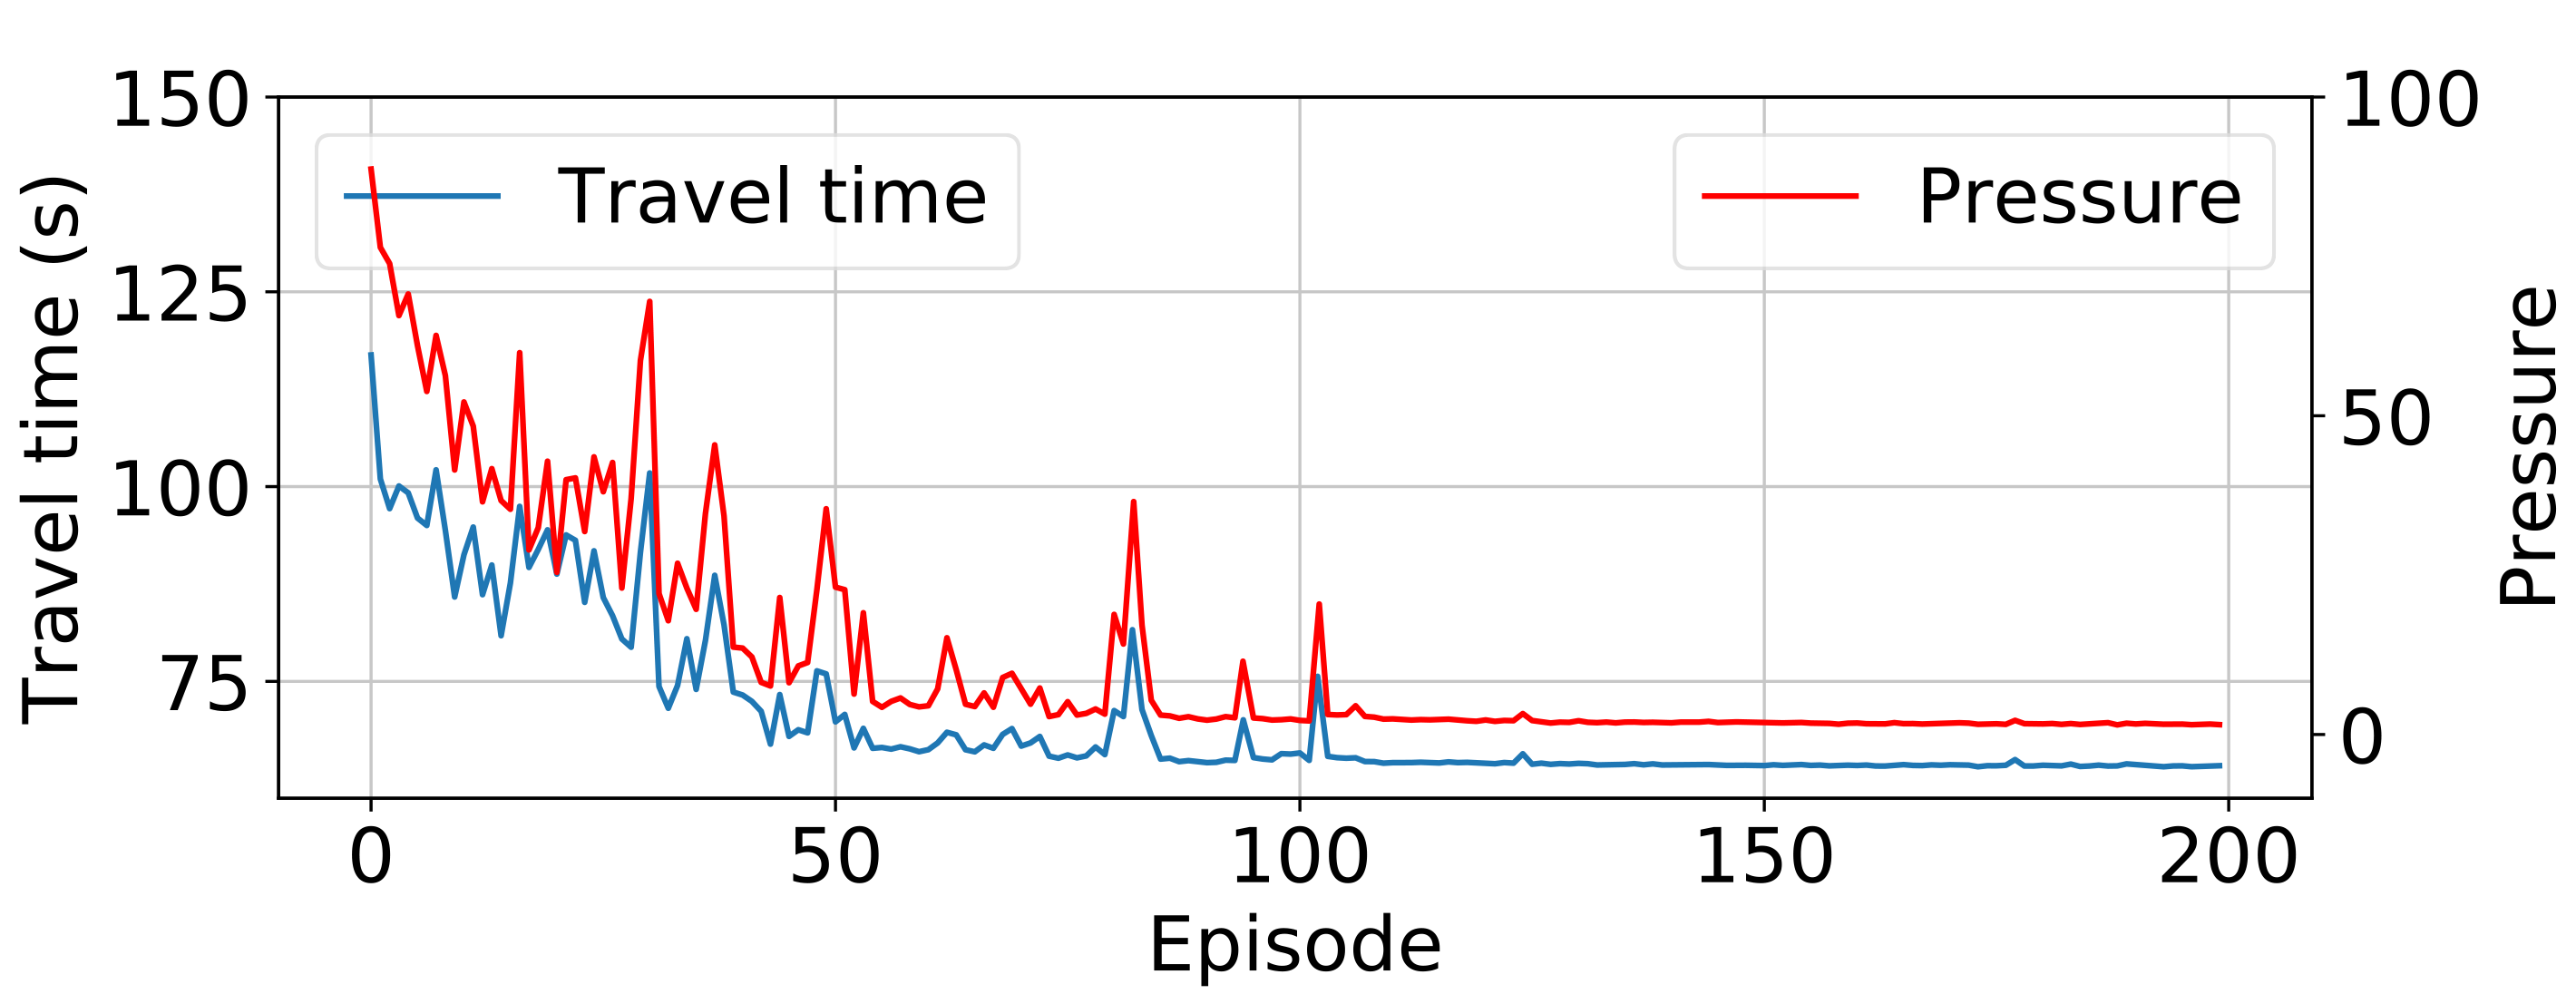
\includegraphics[width=1.0\textwidth]{figures/converg.png} \\
   \end{tabular}
   \end{center}
     \caption{Convergence curve of average duration and our reward design (pressure). Pressure shows the same convergence trend with travel time.}
    \label{fig:convergence}
\end{figure}

\subsection{Performance on Mixed Scenarios}

\subsubsection{Heterogeneous intersections}
We employ our model to two heterogeneous arterials, as is shown in Figure~\ref{fig:heter_inter}. For intersections with 3 legs, we use zero-padding to complete the state. For intersections with different lengths of lanes, our method can handle this well since the state is independent of the lane length. Table~\ref{tab:more-intersection} illustrates the performance of our model against \Maxpressure. 
% The conclusion could be drawn that our model could achieve better performance even when the intersections are heterogeneous.


\begin{figure}[t!]
\centering
   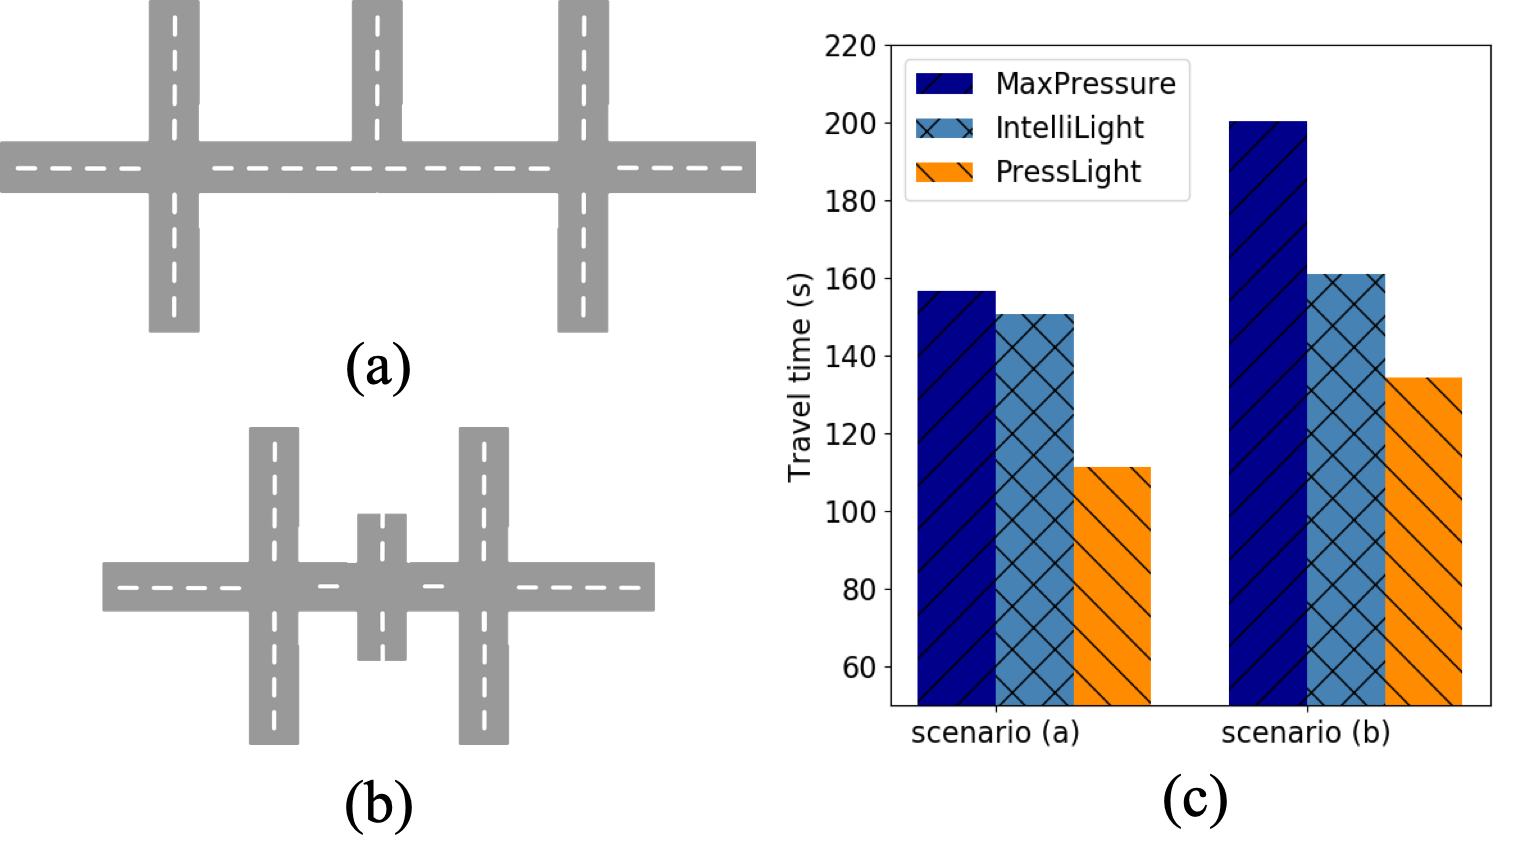
\includegraphics[width=0.8\textwidth]{figures/heter_results.png} 
     \caption{Average travel time of our method on heterogeneous intersections. (a) Different number of legs. (b)  Different length of lanes. (c) Experiment results.}
    \label{fig:heter_inter}
    % \vspace{-2mm}
\end{figure}
% \vspace{-2mm}

\begin{figure}[t!]
\centering
   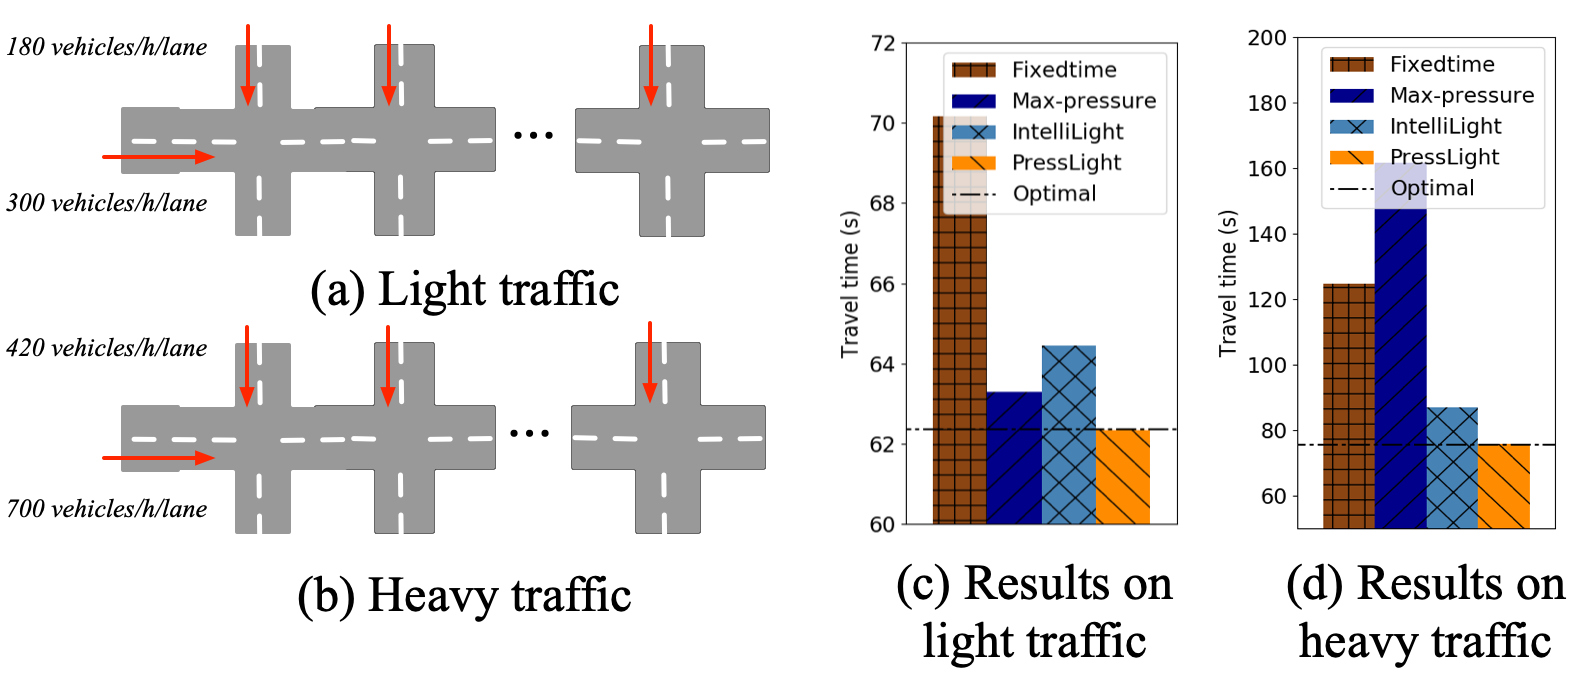
\includegraphics[width=0.9\textwidth]{figures/gw.png} 
     \caption{Performance comparison under uniform unidirectional traffic, where the optimal solution is known (\Greenwave). Only \PressLight can achieve the optimal.}
    \label{fig:optimal}
    % \vspace{-3mm}
\end{figure}

\subsubsection{Arterials with a different number of intersections and network}

\begin{table*}[t!]
\centering
\caption{Average travel time of different methods under arterials with a different number of intersections and network.}
\label{tab:more-intersection}
\begin{tabular*}{\textwidth}{ccccccc}
\toprule
           & \multicolumn{2}{c}{6-intersection arterial} & \multicolumn{2}{c}{10-intersection arterial} & \multicolumn{2}{c}{20-intersection arterial}  \\
           & \HeavyFlat  & \HeavyPeak & \HeavyFlat  & \HeavyPeak  & \HeavyFlat   & \HeavyPeak   \\ \midrule
\Maxpressure        &       262.26        &  225.60  &     129.63         &    129.63     &310.95 &    271.39                \\
\LIT        & 233.17  & 258.33     & 157.84 & 200.96 & 246.88 &  202.30     \\
\PressLight(ours) &  \textbf{160.48}  &  \textbf{184.51}   & \textbf{88.88}   &   \textbf{79.61}  & \textbf{155.84} & \textbf{188.92}           \\  \bottomrule
\end{tabular*}\\
\vfill
\vspace{1cm}
\begin{tabular}{ccc}
\toprule
           &  \multicolumn{2}{c}{Grid network} \\
           &  \HeavyFlat  & \HeavyPeak \\ \midrule
\Maxpressure              &   539.67           &     485.03        \\
\LIT         & 283.21  &    332.53      \\
\PressLight(ours)   \textbf{251.02} &  \textbf{262.46}           \\  \bottomrule
\end{tabular}
\end{table*}


% \begin{table}[tp!]
% \caption{(RQ3) Average travel time of different methods under synthesized traffic with different volumes. }
% \label{tab:RQ3-volume_comparison}
% \begin{tabular}{c|cccc}
% \toprule
%               & \multicolumn{4}{c}{Synthetic traffic }  \\ 
%               & \LightFlat & \LightPeak  & \HeavyFlat& \HeavyPeak  \\ \midrule
% \FT             &  93.29   		&   109.50        &    325.48       &   246.25         \\ 
% \Greenwave      &  98.39    	&  124.09         &   263.36        &   286.85         \\ 
% \Maxpressure    &  74.30       	&  82.37          &   262.26        &   225.60         \\ \hline
% \NIPS           &             	&                 &  525.64         &  757.73          \\
% \LIT      &  65.07       	&  66.77      	  &   233.17        &   258.33         \\ \hline
% \PressLight     &\textbf{59.96}	&  \textbf{61.34} & \textbf{160.48} &  \textbf{184.51} \\ 
% % Improvements &   7.85\%          &  8.13\%           &       5.69\%         &      31
% \bottomrule
% \end{tabular}
% \end{table}

We employ our model to arterials with 6, 10 and 20 intersections under synthetic data. As is shown in Table~\ref{tab:more-intersection},  our model could achieve better performance over conventional transportation method \Maxpressure and reinforcement learning method \LIT even when the number of intersections grows. 

We also test our model a network with 9 intersections ($3\times3$ grid). Table~\ref{tab:more-intersection} shows the experiment results and we can see that \PressLight can outperform \Maxpressure and \LIT under both traffic.

\subsection{Case Study}
Another desirable property of \PressLight is its ability to automatically coordinate the offset between adjacent intersections. To demonstrate this, we show two examples. Under simplified uniform traffic, we show that our model has learned the optimal solution which could be justified by transportation theories. Under the real-world traffic, the learned offset is visualized to reveal this property.
% and to optimize the offset between every two neighboring intersections which is because our designed state could capture the distribution of coming vehicles. To demonstrate this, we show two examples on uniform and real-world traffic.

\subsubsection{Synthetic traffic on the uniform, uni-directional flow}

In this section, we perform experiments on the arterials with six homogeneous intersections under two traffic settings. One is for light traffic (arterial demand: 300 vehicle/hour/lane, side-street demand: 180 vehicle/hour/lane) and one is for heavy traffic (arterial demand: 700 vehicle/hour/lane, side-street demand: 420 vehicle/hour/lane). Both of them are uniform and uni-directional without turning traffic and two phases (\WE for green light on arterial and \SN for green light for side streets) are used for all intersections. Under these simplified scenarios, the optimal solution is known as \Greenwave in transportation area as stated in ~\cite{Roess2011t}. As the optimal solution under these settings, \Greenwave's policy includes the offsets between intersections and the phase split, which requires several prior knowledge to calculate them: The offset $\Delta$ equals to the block length $l$ between two consecutive intersections divided by free-flow speed $v$; the optimal phase split ratio is equal to the ratio of the demand for a designated phase and total demand. In our experiments, $l\approx 300$ m, $v\approx 10$ m/s, hence, the optimal offset should be $\Delta\approx 30$ s, and the optimal phase split should be 1:0.6 (\WE : \SN).

\begin{figure}[t!]
  \centering
	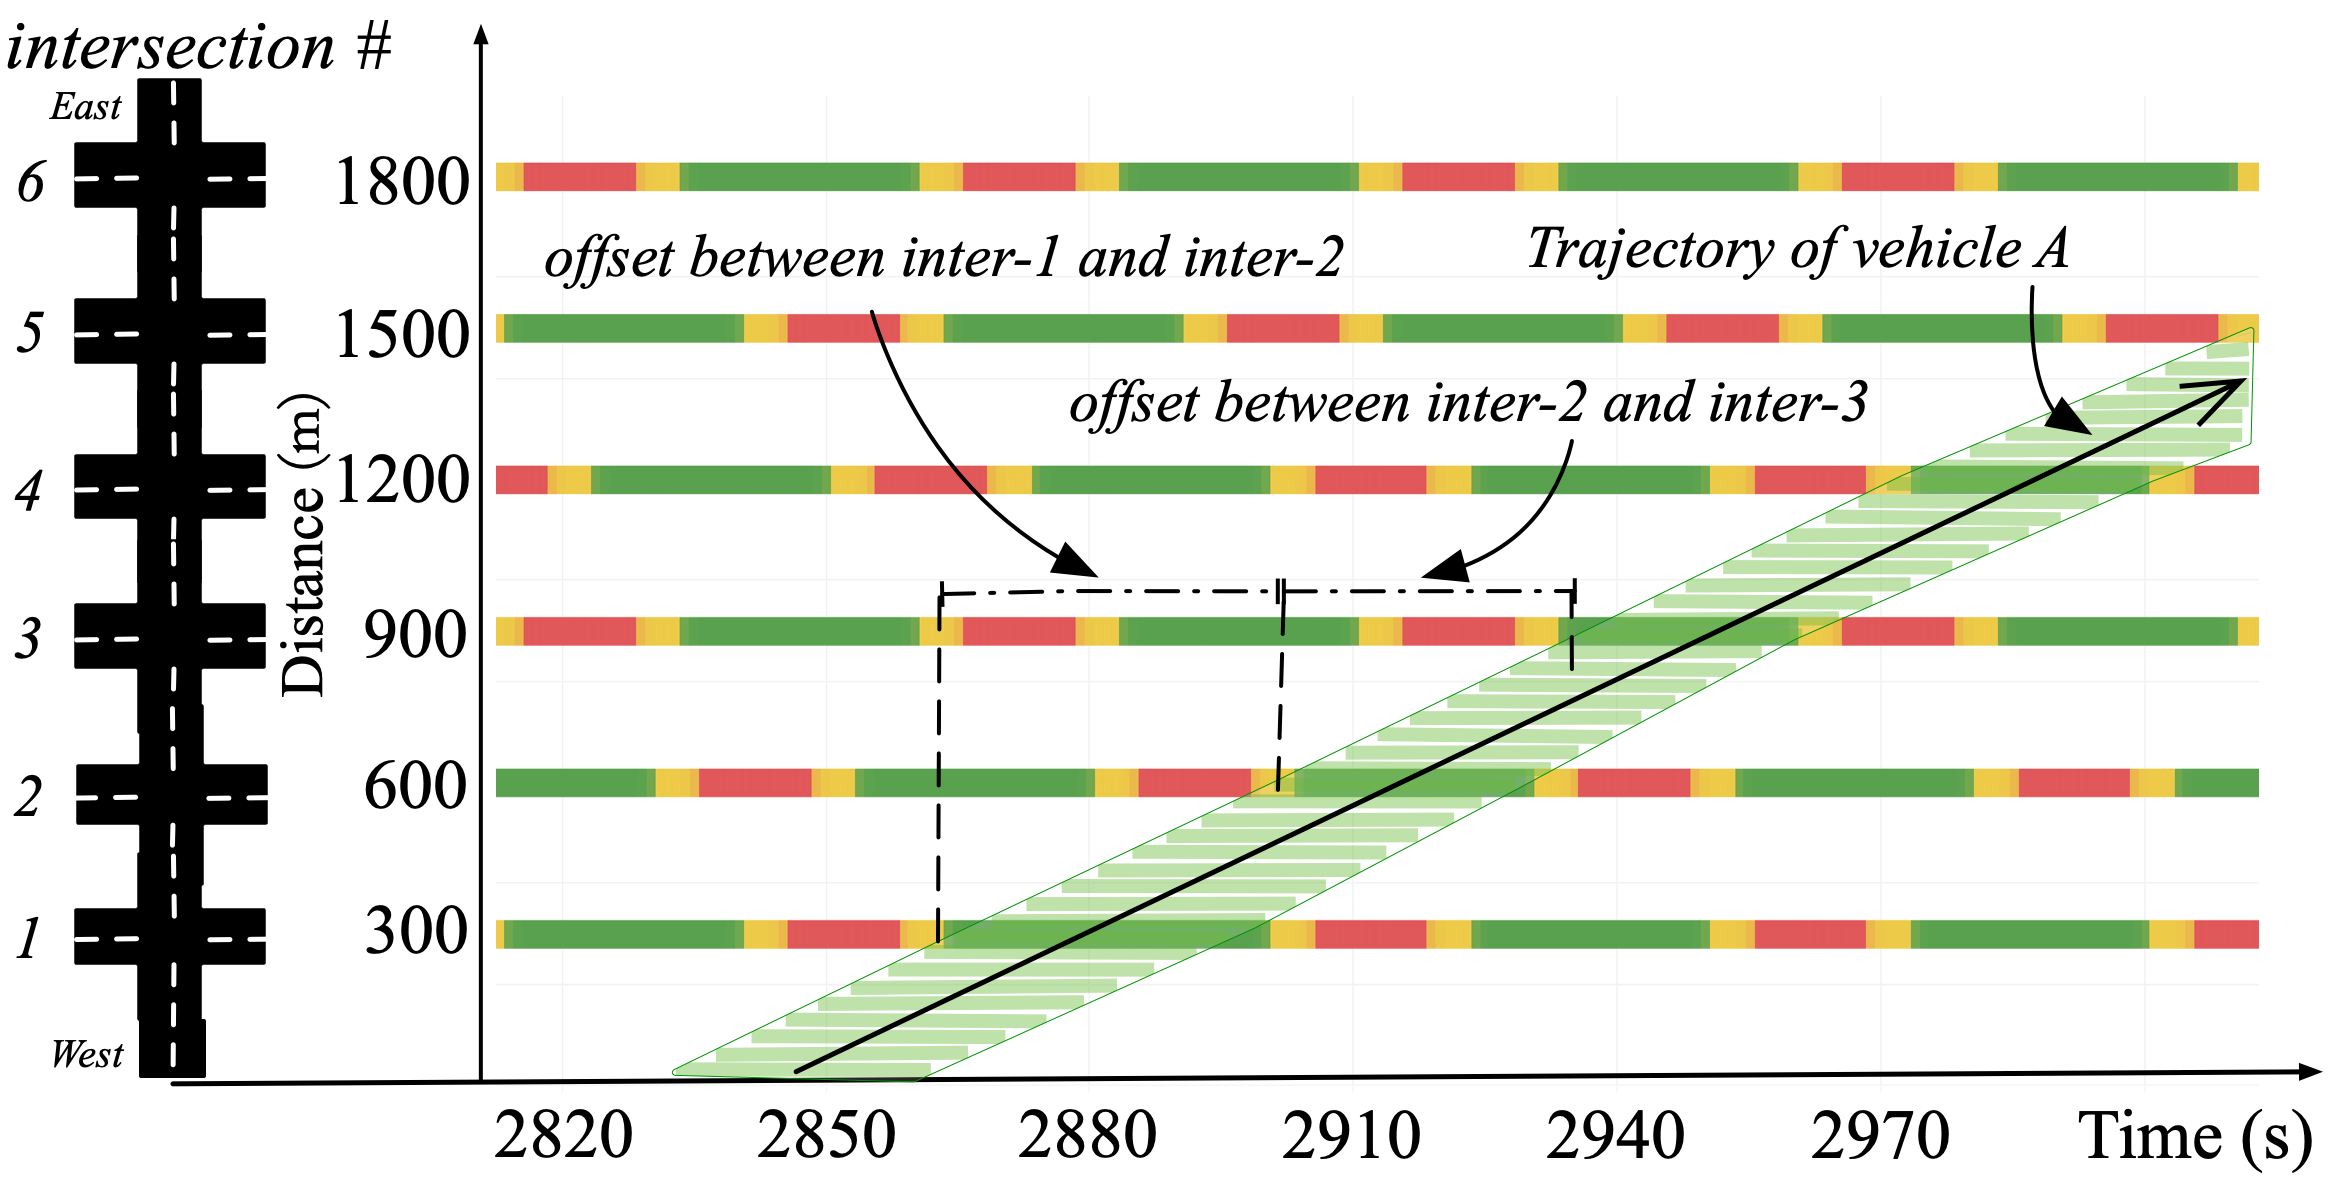
\includegraphics[width=0.8\textwidth]{figures/offset.png}
     \caption{Offsets between intersections learnt by RL agents under uni-directional uniform traffic (700 vehicles/hour/lane on arterial) }   
    \label{fig:case-study}
    % \vspace{-3mm}
\end{figure}

\begin{figure}[t!]
  \centering
  \begin{tabular}{c}
   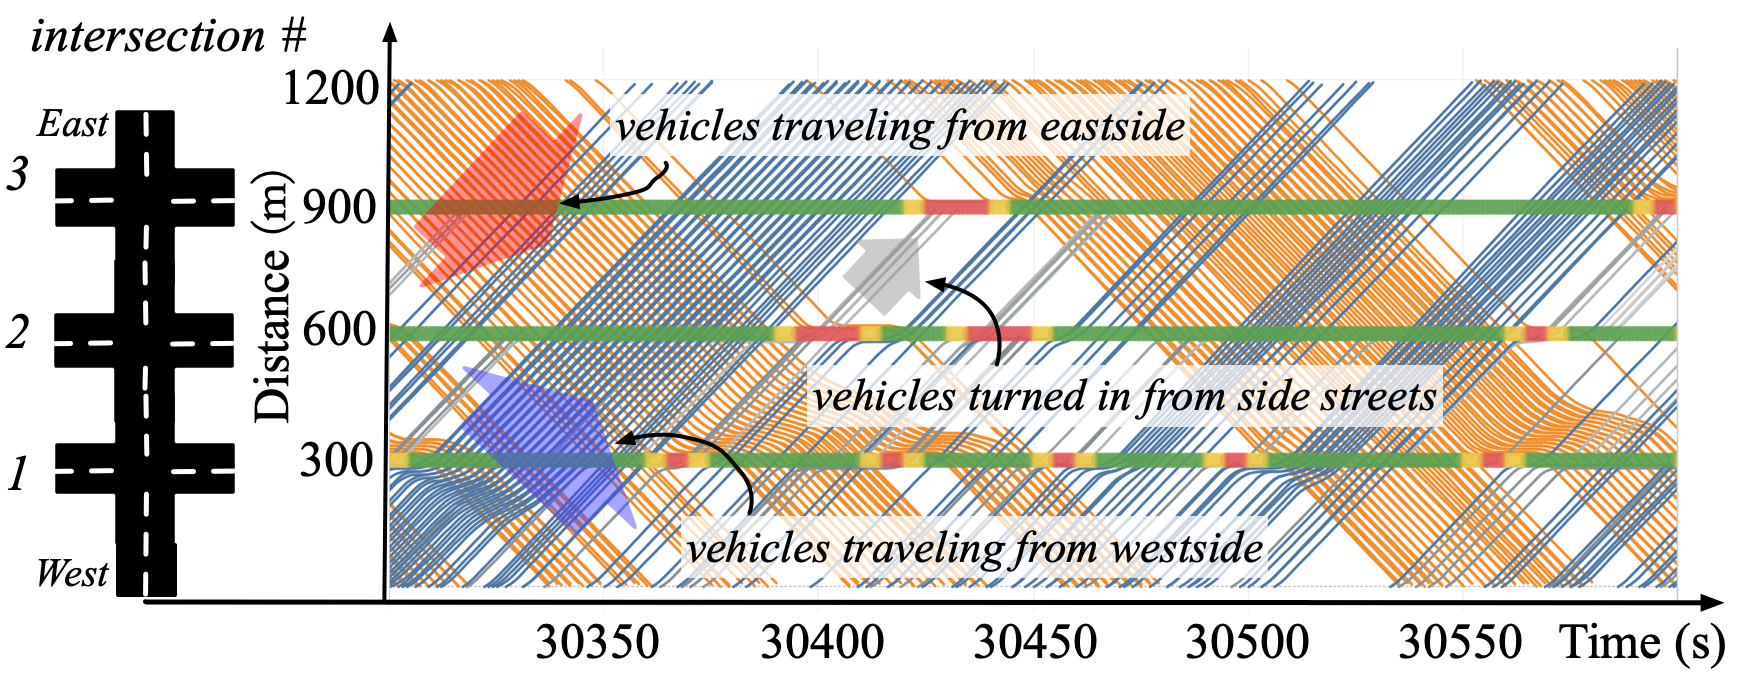
\includegraphics[width=0.8\textwidth]{figures/case_study_1.png} \\
   \end{tabular}
     \caption{Space-time diagram with signal timing plan to illustrate the learned coordination strategy from real-world data on the arterial of Qingdao Road in the morning (around 8:30 a.m.) on August 6th.}
    \label{fig:case-study-real}
    % \vspace{-3mm}
\end{figure}

\paragraph{Performance comparison}
We compared \PressLight with all aforementioned baselines and report their results in Figure~\ref{fig:optimal}. We can find that given \Greenwave is the optimal solution, only our method \PressLight achieves the same performance as \Greenwave in both settings. This demonstrates that our RL agents can learn the optimal policy under these simplified scenarios.


% \begin{figure}[t!]
%   \begin{tabular}{cc}
%   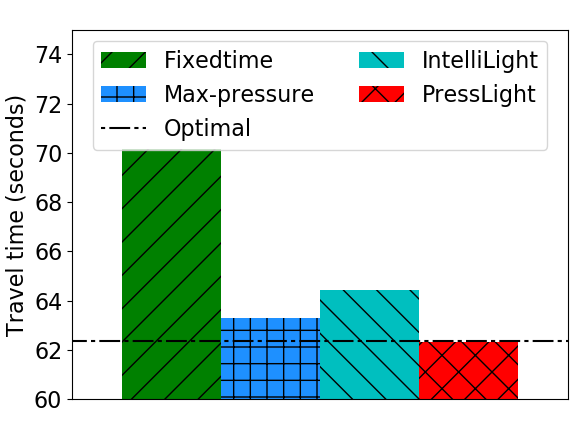
\includegraphics[width=0.22\textwidth]{figures/gw1.png} &
%   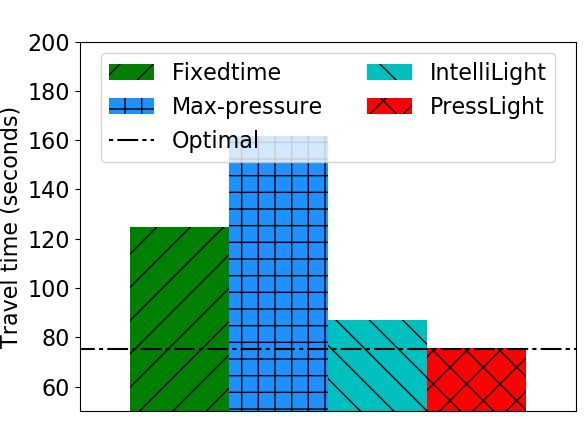
\includegraphics[width=0.225\textwidth]{figures/gw2.png} \\
%   \begin{tabular}[c]{@{}c@{}}(a) Light traffic\end{tabular}&
%   \begin{tabular}[c]{@{}c@{}}(b) Heavy traffic\end{tabular}\\
%   \end{tabular}
%      \caption{Performance comparison between all the methods under uniform unidirectional traffic. Under these situations, the optimal solution is known (\Greenwave). Only our method can achieve the optimal solution.}
%     \label{fig:optimal}
% \end{figure}

\paragraph{Policy learned by RL agents}
We use time-space diagrams to show the trajectories of vehicles and phase plans of traffic signal controllers. In a time-space diagram like Figure~\ref{fig:case-study}, the x-axis is the time and the y-axis is the distance (from a reference point, here we use the westernmost point as the reference point). As it is shown in Figure~\ref{fig:case-study}, there are six bands with green-yellow-red colors indicating the changing phases of six intersections. The black line with an arrow is the trajectory of a vehicle, where the x-axis tells the time and the y-axis tells the location. Vehicles that travel within the green dashed area will experience a green wave. For example, vehicle $A$ enters the system at 2850 second and traveled through 5 intersections at 3000 second, experiencing consecutive green lights during its trip. The slope indicates the speed of the vehicle. 

We have several observations:
\begin{enumerate}[wide,noitemsep,topsep=0pt]
    \item Our RL agents can learn the optimal phase split as \Greenwave.  As is shown in Figure~\ref{fig:case-study}, our method learns optimal phase split (approximately 1:0.6, with 25 seconds of \WE, 15 seconds of \SN, and 10 seconds of yellow light). 
    \item Our RL agents can learn the optimal offset and form a green wave. In Figure~\ref{fig:case-study}, the offset is approximately 30s between two consecutive traffic signals and a green wave can be seen (dashed green area in Figure~\ref{fig:case-study}). This demonstrates that our RL method can learn the optimal policy given by \Greenwave. 
\end{enumerate}

\subsubsection{Real-world traffic in Jinan}

In this section, we make observations on the policies we learned from the real data for the arterial of Qingdao Road ($East$ and $West$ direction) during the morning peak hour (around 8:30 a.m.) on August 6th.  In Figure~\ref{fig:case-study-real}, a time-space diagram is drawn with time on the horizontal axis and distance (from a reference point, here we use the westernmost point on the arterial as the reference point) on the vertical axis. Most of the blue and orange lines are straight, indicating most vehicles on the arterial are not stopped by red lights, which means our method can automatically form a green wave.

\section{Conclusion}
In this chapter, we propose a novel RL method for multi-intersection traffic signal control on the arterials. We conduct extensive experiments using both synthetic and real data and demonstrate the superior performance of our method over the state-of-the-art. Specifically, we draw a connection on the design between reinforcement learning with conventional transportation control methods. It is also the first time the individual RL model automatically achieves coordination along arterial without any prior knowledge. 
 
 We acknowledge the limitations of our model and would like to point out several future directions. In our experiment, we did not model the behavior of vehicles. The behavior of vehicles (e.g., routing) in the real-world may change dynamically in response to traffic lights. Another direction can be reducing the cost of learning. Since RL is learning from trial-and-error, deploying an online updated RL model in real-world could be dangerous and costly.


% \begin{acks}
% The work was supported in part by NSF awards \#1652525, \#1618448, and \#1639150. The views and conclusions contained in this chapter are
% those of the authors and should not be interpreted as representing
% any funding agencies.
% \end{acks}

% %%
% %% The next two lines define the bibliography style to be used, and
% %% the bibliography file.
% \bibliographystyle{ACM-Reference-Format}
% \bibliography{sample-base}

% %%
% %% If your work has an appendix, this is the place to put it.


% \end{document}
% \endinput
%%
%% End of file `sample-sigconf.tex'.

% \input{tex/method}
% \input{tex/experiment}
% \input{tex/conclusion}
% \include
% \include{tex/example}
% \include{tex/faq}
% \include{tex/summary}

\appendix % 使用英文字母对附录编号

% 附录内容,本科学位论文可以用翻译的文献替代。
% \include{tex/app_setup}
% \include{tex/app_eq}
% \include{tex/app_cjk}
% \include{tex/app_log}

\backmatter % 文后无编号部分

% 参考资料
\printbibliography[heading=bibintoc]

% 致谢、发表论文、申请专利、参与项目、简历
% 用于盲审的论文需隐去致谢、发表论文、申请专利、参与的项目
\makeatletter

\ifsjtu@coursepaper
\else

  % "研究生学位论文送盲审印刷格式的统一要求"
  % http://www.gs.sjtu.edu.cn/inform/3/2015/20151120_123928_738.htm

  % 盲审删去删去致谢页
  \ifsjtu@review\relax\else
    %# -*- coding: utf-8-unix -*-
% !TEX program = xelatex
% !TEX root = ../thesis.tex
% !TEX encoding = UTF-8 Unicode
%TC:ignore
\begin{thanks}
I must express my very profound gratitude to my co-workers and advisors for providing me with unfailing support and continuous encouragement throughout my years of study and through the process of researching and writing this thesis.

\end{thanks}
%TC:endignore
         % 致谢
  \fi

  \ifsjtu@bachelor
    % 学士学位论文要求在最后有一个英文大摘要,单独编页码
    %# -*- coding: utf-8-unix -*-
% !TEX program = xelatex
% !TEX root = ../thesis.tex
% !TEX encoding = UTF-8 Unicode
\begin{bigabstract}


\end{bigabstract}
  \else
    % 盲审论文中,发表学术论文及参与科研情况等仅以第几作者注明即可,不要出现作者或他人姓名
    \ifsjtu@review\relax
      \include{tex/pubreview}
      \include{tex/projectsreview}
    \else
      \include{tex/pub}       % 发表论文
      \include{tex/projects}  % 参与的项目
      % \include{tex/patents}   % 申请专利
      \include{tex/resume}    % 个人简历
    \fi
  \fi
\fi

\makeatother

\end{document}
